\section{Arquitectura de Comportamientos}
\label{sec:behaviour_architecture_all}

\subsection{Introducci\'on}
Como mencionamos en las secciones anteriores, el objetivo de \'este trabajo
es desarrollar un robot aut\'onomo y reactivo que recolecte basura en un entorno
estructurado pero din\'amico, debido a que la arena (lugar donde se
mueve el robot) es transitado por personas y est\'a al aire libre.

En esta secci\'on de \emph{Arquitecturas de Comportamientos} detallamos
las acciones que deber\'ia llevar a cabo el robot y c\'omo organizar las mismas
para cumplir la meta de recolectar basura y ser aut\'onomo, es decir, decidir
por s\'i mismo las acciones a realizar en cada momento y ser capaz de mantenerse
cargado para poder continuar recolectando.

En la secci\'on \ref{inv_prev} analizamos papers relacionados con este
desarrollo, desde la forma de organizar los comportamientos, la definici\'on y
composici\'on de los mismos, hasta su implementaci\'on. En la secci\'on
\ref{arq_prop} detallamos la arquitectura elegida para llevar a cabo y
organizar los comportamientos elegidos, y las ventajas y desventajas de usar la
misma. En la secci\'on \ref{comportamientos} detallamos uno por uno los
comportamientos que elegimos para que posea el robot, y sus correspondientes
implementaciones en \emph{pseudo-c\'odigo}. En la secci\'on \ref{odometry}
explicamos que es la odometr\'ia, para qu\'e sirve y qu\'e
ventajas y desventajas tiene usarla. Tambi\'en detallamos el test utilizado
para mejorar la eficiencia de la misma. En la secci\'on \ref{interfaces}
describimos c\'omo estructuramos el controlador del robot para que podamos
ir desarrollando y probando el mismo con un simulador y minimizar el trabajo
al pasarlo a el robot f\'isico. Los resultados de performance y
eficiencia del controlador desarrollado los obtuvimos de la simulaci\'on, y los
mostramos en la secci\'on \ref{results}. Finalmente, en la secci\'on
\ref{comp_conclusion} sacamos conclusiones de los resultados obtenidos y las
dificultades encontradas a lo largo del desarrollo de \'este proyecto final.

\newpage

\subsection{Investigaciones previas}
\label{inv_prev}

A continuaci\'on presentamos trabajos realizados por otros autores
relacionados en alguna forma con el nuestro. Primero damos una breve
descripci\'on del trabajo del otro autor y luego lo comparamos con
nuestro trabajo, analizando similitudes y diferencias entre ambos.

\subsubsection{Desarrollo de comportamientos no triviales en robots reales : 
Robot recolector de basura - Stefano Nolfi \cite{nolfi:evolving}}
En este paper se muestra el uso de un Khepera con el m\'odulo Gripper en una
arena delimitada por paredes para la recolecci\'on de "basura". Dicho robot se
puede ver en la figura \ref{fig:khepera}.
\begin{figure}[htp]
\begin{center}
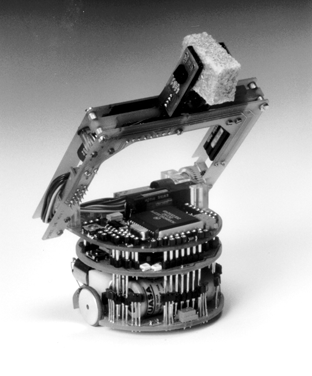
\includegraphics[scale=0.6]{comportamientos/figures/gripperAH.png}
\caption{Robot Khepera con el m\'odulo Gripper}
\label{fig:khepera}
\end{center}
\end{figure}
La base tiene una fuente de luz asociada y el objetivo del robot es llevar
peque\~nos objetos a un lugar de dep\'osito. Se utiliza \emph{aprendizaje por
refuerzo} para asociar las velocidades angulares de las ruedas a los diferentes
tama\~nos de las "basuras". Para obtener el comportamiento deseado se hace uso
de \emph{algoritmos gen\'eticos} y \emph{redes neuronales}. Una vez obtenido el
mismo mediante simulaci\'on en Webots, se lo prob\'o en el Khepera f\'isico.
Comparando el trabajo de Stefano Nolfi con el nuestro podemos realizar las
siguientes comparaciones:
\begin{itemize}

\item{Existencia de un dep\'osito:} Ambos tienen un dep\'osito en el cual dejar
la basura recogida y una forma de identificarla: una fuente de luz usada por
Nolfi y en nuestro trabajo, al llegar al final de una l\'inea marcada sobre la
arena.

\item{Autonom\'ia:} Ambos son aut\'onomos en el sentido que no son manejados
por un humano. En cuanto a la recarga de la bater\'ia, Nolfi no explicita
si es asistida o no; en nuestro caso, el robot se encarga de ir a la base de
recarga una vez detectada la falta de energ\'ia.

\item{M\'etodo de Recolecci\'on:} En el trabajo de Nolfi se utiliza el m\'odulo
��Gripper'' agregado al Khepera. Este m\'odulo simula un brazo con dos dedos.
De \'esta forma, la recolecci\'on se realiza junt\'andolos y la liberaci\'on 
se realiza separ\'andolos. \'Esta forma de recolectar est\'a basada en
el comportamiento humano. Nuestro trabajo se basa m\'as en la actividad humana
para realizar la recolecci\'on, ya que podr\'ia compararse con un recolector
de basura que usa una pala para guardar el residuo en su tacho.

\item{M\'etodo de aprendizaje:} En nuestro trabajo no utilizamos aprendizaje
por refuerzo o algoritmos evolutivos. No es el caso de Nolfi, que
utiliza ambas t\'ecnicas para evolucionar el comportamiento deseado.

\item{Robot Utilizado:} Como mencionamos anteriormente, Nolfi utiliz\'o un
Khepera en la simulaci\'on. En nuestro trabajo utilizamos un E-puck para la
simulaci\'on, una versi\'on nueva del Khepera, pero sin el m\'odulo Gripper.
\begin{figure}[htp]
\begin{center}
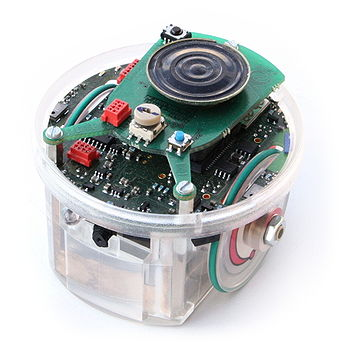
\includegraphics[scale=0.6]{comportamientos/figures/e-puck.png}
\caption{Robot E-puck}
\label{fig:epuck}
\end{center}
\end{figure}

\item{Reconocimiento del objeto a recolectar:} 

\end{itemize}

\subsubsection{Arquitectura de control para un Robot Aut\'onomo M\'ovil -
Neves And Oliveira \cite{Neves97acontrol}}
Neves y Oliveira describen en su trabajo una arquitectura de control basada en
comportamientos para un robot m\'ovil en un ambiente din\'amico, utilizando
muchos aspectos de la arquitectura \emph{Subsumption}(Ver secci\'on
\ref{arq_prop}) propuesta por \emph{Brooks} y que usamos al realizar \'este
proyecto.
\\
La arquitectura propuesta en el paper, o
\emph{Control System Arquitecture}, se basa tambi\'en en la teor\'ia de 
\emph{The Society of Mind}, escrita por \emph{Minsky}\cite{minsky}, donde el sistema es
visto como una sociedad de agentes, cada uno con una competencia particular y
que colaboran entre ellos para ayudar a la sociedad a alcanzar su meta.
La arquitectura est\'a compuesta por tres niveles: un nivel reflexivo, uno
reactivo, y otro cognitivo, aumentando la complejidad al igual que el orden en
que fueron presentados.
\\
El nivel reflexivo incluye aquellos comportamientos innatos, es decir, act\'uan
directamente como est\'imulo-respuesta. El segundo nivel, el reactivo, est\'a
compuesto por agentes que responden r\'apidamente a los est\'imulos ya que
requieren poco nivel de procesamiento. Finalmente, en el nivel cognitivo, se
encuentran los agentes encargados de guiar y administrar los comportamientos
reactivos de forma tal que el robot muestre un comportamiento orientado.
\\
Aunque la arquitectura explicada es similar a la utilizada en nuestro trabajo,
no utilizamos \'esta organizaci\'on de los comportamientos en capas. Sin
embargo, podemos divisar que algunos de los comportamientos que propusimos
corresponden a la primera capa de reflexi\'on, como por ejemplo el evitamiento
de obst\'aculos y otros podr\'ian incluirse en la segunda capa de
comportamientos reactivos, como ser\'ia deambular. Finalmente en la \'ultima
capa estar\'ia el reconocimiento de objectos debido a su gran demanda de
procesamiento.

\subsubsection{Path Planning usando Algoritmos Gen\'eticos - Salvatore Candido
\cite{salvatore}}
En este paper se describe la utilizaci\'on de algor\'itmos gen\'eticos para
resolver el problema de Path Planning. \'Este consiste en armar un
plan, una secuencia de acciones de forma tal que a partir de un punto de origen
se llegue al punto de destino, siguiendo ese plan. Debido a la
componente din\'amica de nuestro trabajo, siempre tratamos de mantener los
comportamientos del robot lo m\'as reactivos posibles, por lo que armar un plan
no ser\'ia la mejor opci\'on a utilizar. Por el contrario, el uso de
algor\'itmos gen\'eticos puede ser una herramienta que se podr\'ia llegar a
usar en una futura continuaci\'on de nuestro trabajo.

\subsubsection{Navegaci\'on predictiva de un robot aut\'onomo - Foka And
Trahanias \cite{Foka02predictiveautonomous}}
La navegaci\'on predictiva nace como una posible soluci\'on al problema de un
robot navegando en un ambiente con muchas personas y obst\'aculos, tal como lo
es el ambiente en el cual navegar\'a nuestro robot.
\\
La forma en que es implementada por los autores es mediante un \emph{POMDP}, es
decir, un proceso de decisi\'on de markov parcialmente observable. Cabe 
destacar estas dos \'ultimas palabras, ya que indican la naturaleza del
ambiente: hay incertidumbre o falta de informaci\'on acerca de ciertas
variables del entorno. En este caso, se utiliza el \emph{POMDP} para manejar
tanto la navegaci\'on del robot como el evitamiento de obst\'aculos, un punto
en que se diferencia de lo que propusimos nosotros, que es tratar el 
\emph{wandering} de forma separada del comportamiento de evitamiento de
obst\'aculos. \'Esto, en parte, se debi\'o a causa de la arquitectura utilizada
ya que desde ese punto de vista, ambos comportamientos tienen niveles de
jerarqu\'ia muy diferentes como se puede ver en la figura
\ref{fig:architecture}.

\subsubsection{Algoritmo de navegaci\'on y evitamiento de obst\'aculos en un
entorno desconocido - Clark Et. al \cite{clark}}
En este paper se presentan dos algoritmos complementarios para la navegaci\'on
en ese tipo de entornos.
\\
El primero consiste en la navegaci\'on y un mapeo del entorno que garantiza una
cobertura completa de una arena cuyas ubicaciones de la paredes no se conocen
\emph{a priori}. Consiste b\'asicamente en un seguimiento de las paredes
complementado por una variaci\'on de \emph{flood filling} para asesgurarse la
cobertura completa de la arena. El algoritmo completo se puede apreciar en la
figura \ref{fig:clark}.
\begin{figure}[htp]
\begin{center}
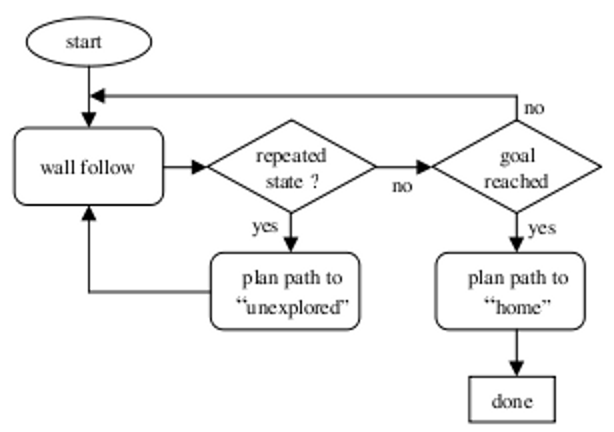
\includegraphics[scale=0.6]{comportamientos/figures/clarkDiagram.png}
\caption{Algoritmo propuesto por Clark Et. al}
\label{fig:clark}
\end{center}
\end{figure}
\\
Un aut\'omata con aprendizaje estoc\'astico es el algoritmo que complementa al
primero, y su objetivo es el evitamiento de obst\'aculos. Para \'esto, se
utiliza un mecanismo de recompensa/castigo de forma tal que se adapten las
probabilidades de las acciones a tomar.
\\
En relaci\'on con nuestro trabajo, hay ciertas similitudes y diferencias,
enumeradas a continuaci\'on:
\begin{itemize}
\item{}Ambos presentan un mecanismo de ``seguimiento de'', en nuestro caso lo
hacemos con l\'ineas, en el paper se utiliza con paredes. Sin embargo,
se utilizan para objetivos diferentes. Nosotros lo usamos para dirigirnos a la
base ya que tratamos de mantener el conocimiento que el robot tiene sobre el
mundo lo m\'as acotado posible.
En el paper se utiliza el mecanismo de seguir las l\'ineas para
obtener un modelo del mundo, algo que puede llegar a servir mucho en ambientes
no tan din\'amicos como el nuestro, raz\'on por la cual no elegimos
implementarlo.
\item{}Tambi\'en coincidimos con la existencia de un m\'etodo para evitar
obst\'aculos. En el paper se implementa como un aut\'omata que va aprendiendo
seg\'un los premios o castigos que recibe. En nuestro caso el comportamiento
es puramente reactivo y reacciona en base a los valores de los sensores de
distancia y no tiene memoria.
\end{itemize}

\newpage
\subsection{Arquitectura propuesta}
\label{arq_prop}
Una arquitectura basada en comportamientos define la forma en que los mismos
son especificados, desde su granularidad (qu\'e tan complejo o simple es un
comportamiento), la base para su especificaci\'on, el tipo de respuesta y la
forma en que se coordinan.
\\
La arquitectura que elegimos para desarrollar nuestro trabajo es
\emph{Subsumption}, desarrollada por Rodney Brooks\cite{brooks} en 1985.
Esta arquitectura est\'a basada en comportamientos puramente reactivos,
rompiendo as\'i con el esquema que estaba de moda en la \'epoca de
\emph{sensar-planear-actuar}. Algunos de los principios propuestos que tuvimos
en cuenta durante el desarrollo de nuestro trabajo son:
\begin{itemize}
\item{}Un comportamiento complejo no es necesariamente el producto de un
complejo sistema de control,
\item{}El mundo es el mejor modelo de \'el mismo,
\item{}La simplicidad es una virtud,
\item{}Los sistemas deben ser construidos incrementalmente.
\end{itemize}
Cada comportamiento es un conjunto de pares est\'imulo-respuesta. Tal como
mostramos en la figura \ref{fig:behaviour}, cada est\'imulo o respuesta puede
ser inhibido o suprimida por otros comportamientos activos. Adem\'as cada
comportamiento recibe una se\~nal de reset, que lo devuelve a su estado
original.
\begin{figure}[htp]
\begin{center}
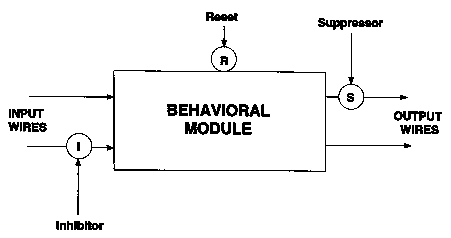
\includegraphics[scale=0.85]{comportamientos/figures/behaviour.png}
\caption{Esquema de comportamiento}
\label{fig:behaviour}
\end{center}
\end{figure}
El nombre \emph{Subsumption} proviene de la forma en que los comportamientos
son coordinados entre s\'i. Hay una jerarqu\'ia donde los comportamientos de la
arquitectura tienen mayor o menor prioridad seg\'un su posici\'on. Los
comportamientos de los niveles inferiores no tienen conocimiento de los
comportamientos de las capas superiores. Gracias a \'esto, se puede plantear
un dise\~no incremental, brindando flexibilidad, adaptaci\'on y paralelismo
al desarrollo e implementaci\'on de los comportamientos.
\\
La idea a seguir es que el mundo sea el principal medio de comunicaci\'on entre
los comportamientos. \'Esto se debe a que la respuesta de un comportamiento
ante un est\'imulo resulta en un cambio en el mundo y, por lo tanto, en la
relaci\'on del robot con el mismo. De \'esta manera, el robot en su pr\'oximo
paso sensar\'a otro estado del mundo.
\\
El procedimiento b\'asico para dise\~nar y desarrollar comportamientos para
robots con esta arquitectura es sencillo:
\begin{enumerate}
\item Especificar cualitativamente la forma en que el robot responde al mundo,
es decir, el comportamiento que realizar\'a.
\item Descomponer la especificaci\'on como un conjunto de acciones disjuntas.
\item Determinar la granularidad del comportamiento, analizando en que nivel de
la jerarqu\'ia existente se encontrar\'a y cuantas acciones disjuntas es
necesario llevar a cabo para el cumplimiento de
la tarea.
\end{enumerate}

Un ejemplo de esta arquitectura se puede observar en la figura 
\ref{fig:subsumptionExample}. En la misma hay 4 comportamientos: Homing,
Pickup, Avoiding y Wandering. Las l\'ineas que entran a cada comportamiento son
los est\'imulos ante los cuales se activan y las salidas son las
se\~nales de respuesta correspondientes. La se\~nal de respuesta de la
arquitectura es la l\'inea que sale por la derecha de la caja (Arquitectura)
que contiene la relaci\'on entre los comportamientos. Puede verse como Homing
inhibe la salida de Pickup ya que su salida entra al supresor (denotado con un
c\'irculo con una S dentro) de la salida de Pickup y por lo tanto, las salidas
de los dem\'as comportamientos, ya que su prioridad es mayor al resto. En el
caso que no est\'en presentes los est\'imulos de Homing, Pickup y Avoiding,
no hay inhibici\'on en la salida de Wandering, y por lo tanto se lleva a cabo
el comportamiento de Wandering.
\begin{figure}[htp]
\begin{center}
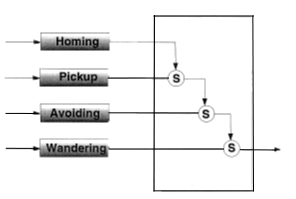
\includegraphics[scale=0.5]{comportamientos/figures/subsumptionExample.png}
\caption{Ejemplo de la arquitectura Subsumption}
\label{fig:subsumptionExample}
\end{center}
\end{figure}


\newpage

\subsection{Comportamientos e implementaciones}
\label{comportamientos}

Una vez que decidimos utilizar la arquitectura explicada en la secci\'on
\ref{arq_prop} para nuestro proyecto, tuvimos que analizar:
\begin{itemize}
\item{}Forma de implementaci\'on de la arquitectura en c\'odigo
\item{}Comportamientos a realizar
\item{}Ordenes de inhibici\'on y supresi\'on entre los mismos
\item{}Forma de implementaci\'on de los mismos
\item{}Orden de implementaci\'on
\end{itemize}

%Detallar que se hizo con cada item
Para implementar la arquitectura decidimos asignarle un $ID$ num\'erico
diferente a cada comportamiento. Tambi\'en tomamos la decisi\'on de elegir como
comportamiento activo en el instante $t$, aquel comportamiento que est\'e
activo en ese instante y tenga mayor $ID$, suprimiendo as\'i el resto de los
comportamientos (con un $ID$ menor) que podr\'ian estar activos.

%Explicar como se relaciona el requerimiento (robot recolector de basura
%autonomo) con los comportamientos que pusimos
El requerimiento de este proyecto es la realizaci\'on de un robot aut\'onomo
que recolecte basura de su entorno din\'amico pero estructuralmente fijo.
De aqu\'i se infieren algunos de los comportamientos que debe tener el robot:
\begin{itemize}
	\item{\emph{Recolectar basura} (\ref{collect_garbage})}
	\item{\emph{Recargar bater\'ia} (\ref{recharge_battery}):} Por ser
		aut\'onomo, debe poder ser capaz de recargarse s\'olo para poder continuar
		con su actividad.
	\item{\emph{Wandering} (\ref{wandering}):} El robot no es controlado por
		control, ya que	es aut\'onomo, por lo que debe poder recorrer el entorno
		por s\'i mismo.
	\item{\emph{Evitamiento de obst\'aculos} (\ref{avoid_obstacles}):} Debido a
		la naturaleza del entorno, el robot debe ser capaz de navegar sin chocarse
		contra los l\'imites del entorno ni con las personas que circulan por el
		mismo.
\end{itemize}

El comportamiento de recolectar basura y el requerimiento de la autonom\'ia
llevan a su vez a la aparici\'on de m\'as comportamientos: \emph{Descargar
basura} (\ref{unload_garbage}) e \emph{Ir hacia basura} (\ref{go_to_garbage}).
\\
La figura \ref{fig:architecture} muestra los comportamientos implementados y
su orden de jerarqu\'ia. Se puede ver que hay m\'as comportamientos de los
detallados anteriormente. \'Esto se debi\'o a que la forma en que se
implementamos los comportamientos b\'asicos del robot nos requiri\'o el
desarrollo de comportamientos auxiliares.
\\
\begin{figure}[htp]
\begin{center}
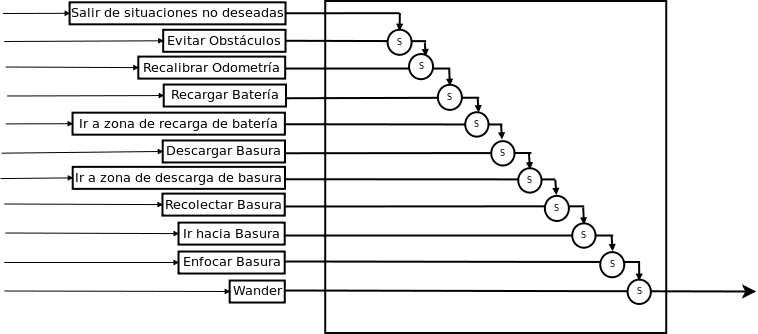
\includegraphics[scale=0.5]{comportamientos/behavioursArchitecture2.png}
\caption{Arquitectura de Comportamientos}
\label{fig:architecture}
\end{center}
\end{figure}
\\
Primero implementamos \emph{Wandering} debido a, en una primera aproximaci\'on,
la sencillez del mismo. Luego implementamos \emph{Evitamiento de obst\'aculos}
para lograr que el robot pueda navegar sin problemas por el arena. Como el
comportamiento de recolectar e ir hacia la basura dependend\'ia del m\'odulo
de reconocimiento de objetos y el mismo estaba siendo desarrollado en paralelo,
se decidi\'o implementar el comportamiento de \emph{Recargar bater\'ia} y
\emph{Descargar basura}. Una vez que tuvimos la primera implementaci\'on
funcional del reconomiento de objetos, procedimos a desarrollar
\emph{Ir hacia basura} y \emph{Recolectar Basura}.
\\
A continuaci\'on detallamos los comportamientos indicados en la figura
\ref{fig:architecture}, as\'i como la implementaci\'on en
\textit{pseudo-codigo} de los mismos y detalles tenidos en cuenta para la
realizaci\'on de los mismos.
%A continuacion vamos a explicar cada comportamiento.....

\subsubsection{Wandering}
\label{wandering}

\paragraph{Detalle del comportamiento} 
Por ser el comportamiento que menor jerarqu\'ia tiene (Ver figura
\ref{fig:architecture}), es el \'unico comportamiento que est\'a activado
ante la ausencia de un est\'imulo, asegurandonos que siempre haya por lo menos
un comportamiento activo.
\\
En una primer aproximaci\'on de \emph{Wandering}, s\'olo nos preocupamos por
ir hacia adelante ya que eventualmente, el robot encuentra un obst\'aculo y
realiza un giro cambiando la direcci\'on del robot.
\\
Los resultados de la simulaci\'on nos indicaron que el robot no recorr\'ia
ciertas zonas o las recorr\'ia despu\'es de un largo tiempo, lo que nos llev\'o
a un segundo approach. El mismo tiene en cuenta el hecho de que el robot posee
una c\'amara y por lo tanto se puede llevar un seguimiento de los lugares que
m\'as recientemente visit\'o o las zonas que hace mucho tiempo no visita.
\\
\'Este approach, en cierta forma, genera un modelo del mundo, un hecho que
conflict\'ua con uno de los principios propuestos a seguir en la secci\'on
\ref{arq_prop}. Para minimizar el conflicto, decidimos mantener al m\'inimo la
informaci\'on almacenada para el funcionamiento del algoritmo, es decir, por
cada zona de arena s\'olo mantenemos el timestamp de la \'ultima vez que el
robot la visit\'o.

\paragraph{Implementaci\'on del comportamiento}

La implementaci\'on del segundo approach, en \emph{pseudo-c\'odigo} es la
siguiente:
\begin{verbatim}
por cada paso
    zona = pedir_zona_vista(camara)
    marcar_zona_como_vista(modelodelmundo,zona)
    ultimazonavisitada = pedir_ultima_zona_visitada(modelodelmundo)
    velocidades = calcular_velocidades_de_ruedas(ultimazonavisitada)
    poner_velocidades_en_ruedas(velocidades)
\end{verbatim}
Para obtener la zona vista por la c\'amara, necesitamos de la altura $C_h$ a la
cual est\'a ubicada la c\'amara en el robot, el campo de visi\'on (de ahora en
adelante \emph{Field of View o FOV}) horizontal $FOV_h$ o vertical $FOV_v$ y
el \'angulo de inclinaci\'on de la c\'amara $ac$. Viendo la figura 
\ref{fig:angleCamera} podemos ver que:

\begin{figure}[htp]
\begin{center}
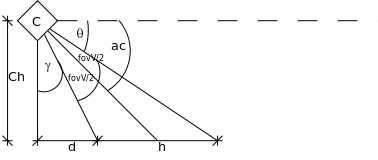
\includegraphics{comportamientos/angleCamera.png}
\caption{Diagrama de posici\'on de la c\'amara}
\label{fig:angleCamera}
\end{center}
\end{figure}

\begin{eqnarray}
ac = \frac{FOV_v}{2} + \theta\\
\gamma + FOV_v + \theta = \frac{\pi}{2}\\
\tan(\gamma) = \frac{d}{C_h}\\
\tan(\gamma+FOV_v) = \frac{d+h}{C_h}
\end{eqnarray}

%En caso de no disponer del $FOV_v$, el mismo se puede obtener de:
%\begin{equation}
%FOV_v = \atan(\frac{ \tan(\frac{FOV_h}{2}) * height}{width} * 2)\\
%\end{equation}
Organizando las ecuaciones, podemos deducir que:

\begin{eqnarray}
\gamma = \frac{\pi}{2} + ac - \frac{FOV_v}{2}\\
\label{eqn:distance_d}
d = \tan(\gamma) * C_h \\
\label{eqn:distance_dh}
d+h = \tan(\gamma+FOV_v) * C_h
\end{eqnarray}

Por lo que obtenemos el \'angulo hasta el inicio de la im\'agen de la c\'amara
$\gamma$ y como consecuencia, la distancia $d$ desde la posici\'on de la
c\'amara hasta el inicio de la im\'agen y $d+h$, la distancia desde la
posici\'on de la c\'amara hasta el final de la im\'agen. Usando \'estos datos,
la posici\'on del robot $P$ y bas\'andonos en la figura \ref{fig:zoneCamera},
podemos obtener los puntos $A$, $B$, $C$ y $D$ del trapezoide que determina la
zona que ve la c\'amara.

\begin{figure}[htp]
\begin{center}
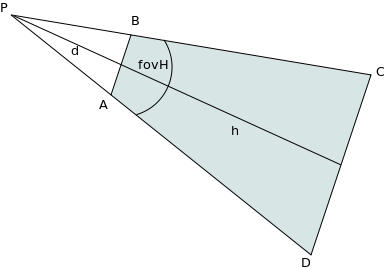
\includegraphics[scale=0.5]{comportamientos/rectangleWander.png}
\caption{Zona vista por la c\'amara}
\label{fig:zoneCamera}
\end{center}
\end{figure}

\subsubsection{Enfocar Basura}
\label{focus_garbage}
Una vez que el m\'odulo de detecci\'on de objetos reconoce algo como basura
(ver secci\'on \ref{algoritmo_vision}), hay que elegir
la forma en que se va a la basura. En la figura \ref{fig:papproachgoto} se
puede ver un primer approach de hacer \'esto. Consiste en primero enfocar la
basura de forma tal que la misma quede en el centro de la imagen de la
c\'amara. De aqu\'i surge el comportamiento \emph{Enfocar Basura}.
\\
Un segundo approach (Figura \ref{fig:sapproachgoto}) no consiste en enfocar la
basura, sino que se idea un arco hacia la misma. \'Esto requiere que se seteen
las velocidades correspondientes a las ruedas de forma tal que la trayectoria
del robot describa dicho arco. Con este segundo approach no existir\'ia el
comportamiento que se est\'a describiendo.
\\
Dado que el primer approach es levemente m\'as simple de implementar, y
teniendo en cuenta el principio enunciado en la secci\'on \ref{arq_prop}
\emph{``La simplicidad es una virtud''}, elegimos implementar el mismo, a
pesar de tener un posible inconveniente, como se puede ver en la figura
\ref{fig:papproachgotoproblem}.
\\
Cuando hay una basura en alguna esquina superior de la imagen de la c\'amara,
y el robot gira sobre s\'i mismo para enfocarla, la basura puede llegar a
perderse por el fondo de la imagen. \'Esto se debe a que la distancia hacia
dichas esquinas es mayor a la distancia hacia el centro del borde superior de
la imagen (Ver figura \ref{fig:zoneCamera}). Decimos que es un ``posible''
problema, ya que una vez que se pierde de vista la basura, el robot no
enfocar\'a m\'as debido a que el est\'imulo desapareci\'o, pero si luego se
dirige hacia adelante (por la activaci\'on de alg\'un otro comportamiento), la
basura volver\'a a aparecer en la imagen, sin desaprovechar la oportunidad de
recogerla.

\begin{figure}[htp]
\begin{center}
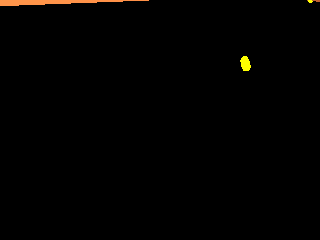
\includegraphics[scale=0.5]{comportamientos/basura.png}
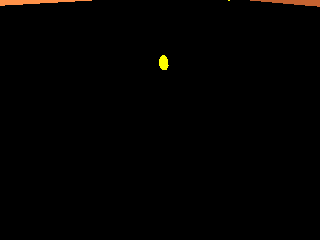
\includegraphics[scale=0.5]{comportamientos/basuraenfocada.png}
\caption{Primer approach de ir a la basura}
\label{fig:papproachgoto}
\end{center}
\end{figure}

\begin{figure}[htp]
\begin{center}
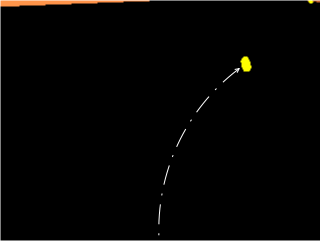
\includegraphics[scale=0.5]{comportamientos/basuraAlt.png}
\caption{Segundo approach de ir a la basura}
\label{fig:sapproachgoto}
\end{center}
\end{figure}

\begin{figure}[htp]
\begin{center}
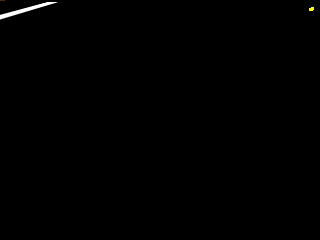
\includegraphics[scale=0.3]{comportamientos/esquina.png}
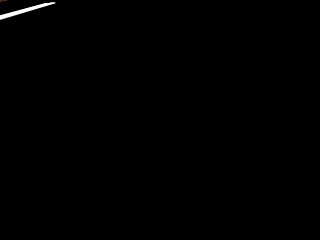
\includegraphics[scale=0.3]{comportamientos/frentemuylejos.png}
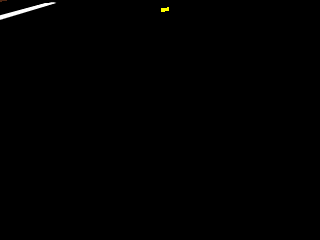
\includegraphics[scale=0.3]{comportamientos/frentelejos.png}
\caption{Posible inconveniente con el primer approach de ir a la basura}
\label{fig:papproachgotoproblem}
\end{center}
\end{figure}

\paragraph{Detalle del comportamiento}
El approach elegido, entonces, se puede describir como:
\begin{itemize}
\item Si la basura est\'a a la izquierda de la im\'agen, se debe girar hacia la
			izquierda
\item Si la basura est\'a a la derecha de la im\'agen, se debe girar hacia la
			derecha
\item Si la basura est\'a en el centro, ya est\'a enfocada
\end{itemize}

%En el caso que haya m\'as de una basura elegimos la m\'as cercana, usando
%c\'alculos detallados a continuaci\'on.
\paragraph{Implementaci\'on del comportamiento}
\label{focus_garbage:impl}
El comportamiento sigue el siguiente \emph{pseudo-codigo}:
\begin{verbatim}
por cada paso
    lista_de_basuras = obtener_lista_de_basuras(modulodereconocimiento)
    basura_mas_cercana = elijo_basura_mas_cercana(lista_de_basuras)
    angulo_a_basura = obtener_angulo(basura_mas_cercana)
    velocidad = VELOCIDAD_BASE * (abs(angulo_a_basura) / (PI/2))
               + VELOCIDAD_BASE_MINIMA

    si angulo_a_basura < 0 entonces
        veloc_izq = -velocidad
        veloc_der = velocidad
    sino
        veloc_izq = velocidad
        veloc_der = -velocidad
    fin_si
    poner_velocidades_en_ruedas(veloc_izq,veloc_der)
\end{verbatim}

Se puede ver que la velocidad de giro del robot es proporcional al m\'odulo del
\'angulo que hay hacia la basura, logrando enfocar m\'as r\'apido cuando el
\'angulo es mayor y tener mayor precisi\'on cuando el \'angulo es m\'as chico,
adem\'as de tener mayor rapidez de enfoque y precisi\'on que si la velocidad de
giro fuera constante.
\\

%%Para obtener el \'angulo y distancia hacia una basura....
%%pasamos de una posicion (x,y) en la imagen a una posicion
%(x,z) en el mundo. teniendo nuestra posicion P, podemos
%calcular la distancia y el angulo
\subsubsection{Ir a Basura}
\label{go_to_garbage}
Luego de la elecci\'on de la forma que se resuelve la situaci\'on de encontrar
una basura (ver \ref{focus_garbage}), el comportamiento de ir a basura es
trivial, ya que la basura, luego de ser enfocada, est\'a delante del robot y lo
\'unico que basta es ir hacia adelante.

\paragraph{Detalle del comportamiento}
El est\'imulo necesario para que este comportamiento est\'e presente est\'a
dado por dos condiciones:
\begin{enumerate}
\item El m\'etodo de reconociemiento de objetos reconoci\'o una basura
\item La basura se encuentra en un entorno del medio horizontal de la imagen de
la c\'amara
\end{enumerate}

\paragraph{Implementaci\'on del comportamiento}
\label{go_to_garbage:impl}
\begin{verbatim}
por cada paso
    distancia = obtener_distancia_a_basura(modulodereconocimiento)
    coeff = (distancia - DIST_MIN)/(DIST_MAX - DIST_MIN)
    veloc_der = VELOCIDAD_MIN*(1 - coeff) + coeff*VELOCIDAD_MAX
    veloc_izq = veloc_der
    poner_velocidades_en_ruedas(veloc_izq,veloc_der)
\end{verbatim}

Al igual que en la implementaci\'on del comportamiento \ref{focus_garbage:impl},
las velocidades que se le otorgan a las ruedas dependen de la distancia
hacia la basura, de forma tal que si una basura est\'a muy lejos, la velocidad
sea mayor y a medida que se va acercando, vaya disminuyendo linealmente.

Dado que la basura se encuentra en un entorno del eje Y en la imagen (Ver figura
\ref{fig:image_coord_conv}b) cometemos un error muy peque\~no al estimar la
distancia a la basura como si estuviera sobre el mismo (asumiendo que la
coordenada X de la basura en la imagen es 0).

Como muestran las figuras \ref{fig:image_coord_conv} y \ref{fig:angleCamera},
el \'angulo vertical hacia el punto m\'as alto de la imagen $(0,C_{rh})$ es 
$\gamma+FOV_v$ y hacia el m\'as bajo, $(0,0)$, el \'angulo es $\gamma$.
De las ecuaciones \eqref{eqn:distance_d} y \eqref{eqn:distance_dh} sabemos
las distancias a los puntos $(0,0)$ (DIST\_MIN) y $(0,C_{rh})$ (DIST\_MAX). 
Entonces, para obtener la distancia $dy$ hacia el punto $(0,y)$ basta con
calcular:
\begin{eqnarray}
y_{angle} = FOV_v * \frac{y}{h} \\
dy = \tan(\gamma + y_{angle}) * C_h \\
\end{eqnarray}

donde $y_{angle}$ es la proporci\'on de $FOV_v$ hacia $y$.
\begin{figure}[htp]
\begin{center}
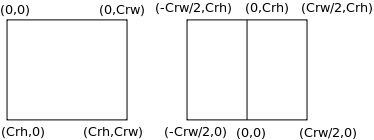
\includegraphics[scale=0.5]{comportamientos/imageCoordsConvertion.png}
\caption{Conversi\'on de coordenadas de imagen de c\'amara}
\label{fig:image_coord_conv}
\end{center}
\end{figure}

\subsubsection{Recolectar Basura}
\label{collect_garbage}
Una vez que el robot llego a estar posicionado para recolectar la basura
deseada, el comportamiento de \emph{recolectar basura} se activa. El mecanismo
para \'esto fue cambiando a lo largo del desarrollo del proyecto.
\\
En un principio pensamos en usar una rampa interna dentro del robot, de forma
tal que la basura suba esa rampa para luego caer en un dep\'osito de basura
interno al robot. Por problemas con la simulaci\'on de este procedimiento, se
busc\'o otro mecanismo.
\\
El mecanismo que elegimos para usar en la simulaci\'on fue el siguiente:
\begin{itemize}
	\item El robot tiene un servo en su parte posterior (debajo de la c\'amara)
	\item Dos paredes delimitan el espacio a lo largo de la direcci\'on que une
			el centro del robot con el servo anteriormente mencionado.
\end{itemize}

\paragraph{Detalle del comportamiento}
La activaci\'on de \emph{recolectar basura} depende de 3 condiciones:
\begin{itemize}
	\item Las dos condiciones impuestas para \emph{ir a basura}
	\item La distancia a la basura elegida para ser recolectada debe ser menor a
			un umbral.
\end{itemize}

Aqu\'i se puede observar que tan importantes son los comportamientos anteriores
para que el robot logre recolectar la basura.
\\
Es importante la elecci\'on del umbral: un valor muy chico puede llevar a que el
comportamiento no se active porque la basura ya no est\'a m\'as en la imagen.
Por otro lado, un valor muy grande causar\'ia que el robot se disponga a
recolectar una basura que est\'a muy lejos y podr\'ia llegar a moverse por
cuestiones propias del ambiente, llevando as\'i a una innecesaria activaci\'on
del comportamiento.

\paragraph{Implementaci\'on del comportamiento}
El \emph{pseudo-codigo} de este comportamiento es el siguiente:

\begin{verbatim}
    distancia = obtener_distancia_a_basura(modulodereconocimiento)
    levantar(servo_delantero)
    recorrerdistancia(distancia)
    cerrar(servo_delantero)
\end{verbatim}

La distancia hacia la basura es obtenida de la misma forma que en la secci\'on
\ref{go_to_garbage:impl}. Levantar y cerrar el servo consiste en setear su
posici\'on en $\frac{\pi}{2}$ y $0$ respectivamente. Para calcular la distancia
recorrida se utiliz\'o la distancia entre la posici\'on del robot en el
instante $t$, $P_r(t)$ y el instante $t+1$, $P_r(t+1)$, ambas dadas por la
odometr\'ia (Ver secci\'on \ref{odometry}). Las diferentes etapas de la
recolecci\'on de una basura se puede ver en la figura \ref{fig:recollection}.

\begin{figure}[htp]
\begin{center}
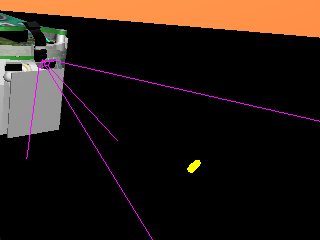
\includegraphics[scale=0.25]{comportamientos/collect1.png}
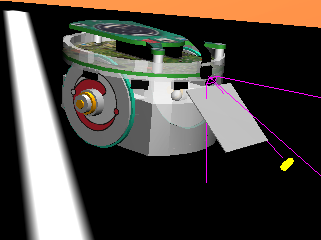
\includegraphics[scale=0.25]{comportamientos/collect2.png}
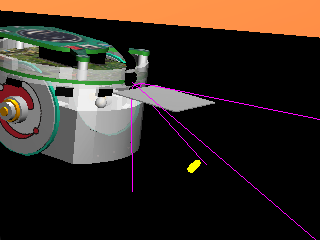
\includegraphics[scale=0.25]{comportamientos/collect3.png}
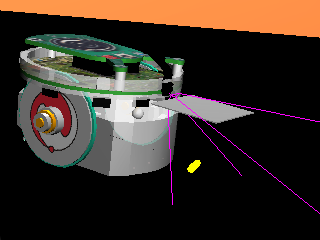
\includegraphics[scale=0.25]{comportamientos/collect4.png}
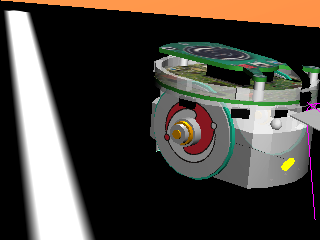
\includegraphics[scale=0.25]{comportamientos/collect5.png}
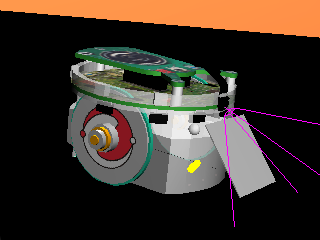
\includegraphics[scale=0.25]{comportamientos/collect6.png}
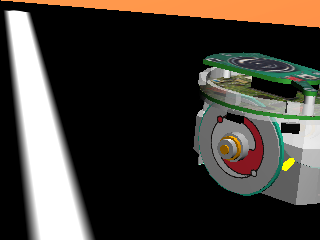
\includegraphics[scale=0.25]{comportamientos/collect7.png}
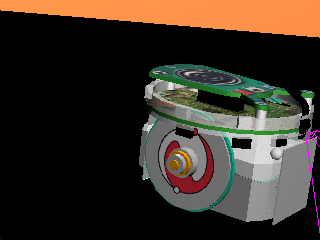
\includegraphics[scale=0.25]{comportamientos/collect8.png}
%
\includegraphics[scale=0.3]{comportamientos/unk.jpg}
\caption{Etapas de recolecci\'on de basura}
\label{fig:recollection}
\end{center}
\end{figure}


\subsubsection{Ir a zona de descarga de basura}
\label{go_to_unload_zone}
Como la capacidad del dep\'osito interno de basura del robot tiene un l\'imite, 
surge como necesidad que el robot sea capaz de ir hacia una zona donde
descargar\'a la basura que contiene, surgiendo as\'i el est\'imulo necesario
para la activaci\'on de este comportamiento.
\\
Para ir hacia dicha zona, decidimos imponerle una condici\'on al
entorno donde el robot actuar\'a. \'Esta condici\'on consiste en poner l\'ineas
de forma tal que si el robot sigue la misma, lo lleve al lugar donde se
encuentra la zona de descarga.
\\
Por lo tanto, para dirigirse a la zona de descarga de basura, es necesario:
\begin{itemize}
	\item Buscar la l\'inea e ir a la misma
	\item Entrar a la l\'inea, de forma tal que el robot y la l\'inea est\'en
				alineados
	\item Seguir la l\'inea
\end{itemize}
Siguiendo con la idea que es mejor descomponer un comportamiento complejo en
otros m\'as simples, decidimos separar el comportamiento de \emph{Ir a zona de
descarga de basura} en 3 comportamientos m\'as simples: \emph{Buscar l\'inea},
\emph{Entrar a la l\'inea} y finalmente \emph{Seguir la l\'inea}.

\paragraph{Buscar l\'inea}
\label{find_line}
Inicialmente, hab\'iamos dispuesto las l\'ineas de forma tal que sigan los
l\'imites de la arena. Entonces para buscar la l\'inea tuvimos que calcular
para cada l\'inea cu\'al es la distancia hacia la misma, luego elegir ir a la
que menor distancia hab\'ia. Adem\'as de ser costoso, este approach ten\'ia un
problema: a veces suced\'ia que al ir hacia una l\'inea, la distancia hacia
otra pasaba a ser m\'as corta y \'esta \'ultima pod\'ia estar m\'as lejos de la
zona de recarga que la primera.
\\
Luego repensamos el problema y nos dimos cuenta que el objetivo era llegar a la
zona de descarga, por lo que decidimos dejar s\'olo 2 las l\'ineas que se
encuentran cerca de la misma, como se puede apreciar en la figura
\ref{fig:arenafinal}. La zona de descarga se ubica cerca de donde se encuentra
el cilindro de color verde.
\\
Para distinguir si el robot est\'a en una l\'inea o no, utilizamos sensores de
piso dispuestos como se muestra en la figura \ref{fig:floorSensors}. Los
sensores se encuentran a una distancia $Fsd$ del centro del robot sobre el eje
$Y$ y los de los costados a una distancia $Fss$ del eje $Y$. La distancia del
sensor del medio hacia el centro del robot es $a$, mientras que la distancia
hacia un sensor del costado es $Fsl = \sqrt{Fsd^2 + Fss^2}$.

\begin{figure}[htp]
\begin{center}
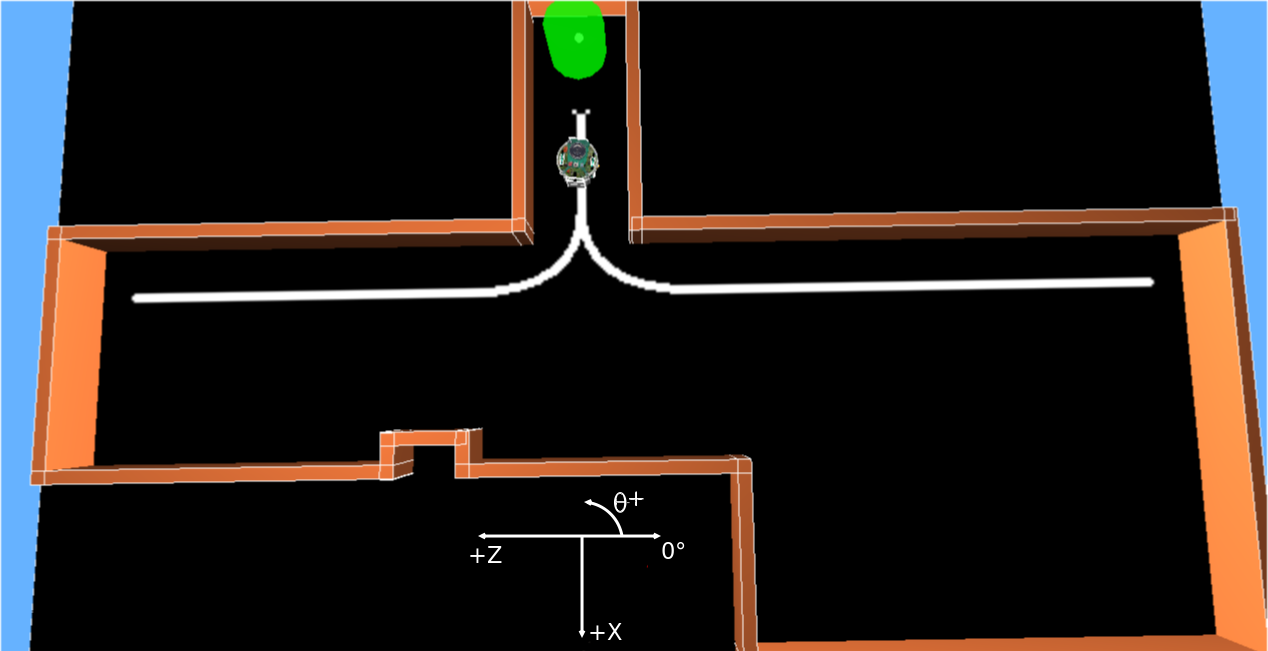
\includegraphics[scale=0.3]{comportamientos/arenafinal.png}
\caption{Arena de simulaci\'on y ejes de coordenadas}
\label{fig:arenafinal}
\end{center}
\end{figure}

\begin{figure}[htp]
\begin{center}
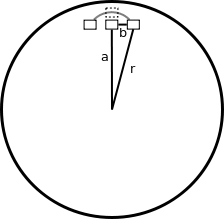
\includegraphics[scale=1.0]{comportamientos/floorSensors.png}
\caption{Disposici\'on de sensores de piso}
\label{fig:floorSensors}
\end{center}
\end{figure}

\subparagraph{Detalle del comportamiento}
La decisi\'on de dejar s\'olo dos l\'ineas, acompa\~nada por la elecci\'on de
la ubicaci\'on de la zona de descarga, nos facilit\'o la composici\'on de
\'este comportamiento.
\\ Como se ve en la figura \ref{fig:arenafinal}, para ir a la l\'inea se debe
girar hasta tener un \'angulo de $\frac{\pi}{2}$ y luego ir hacia adelante.

%Describir la eleccion de las distancias de las lineas hacia las paredes

\subparagraph{Implementaci\'on del comportamiento}
El \emph{pseudo-codigo} de este comportamiento es sencillo, ya que
no requiere c\'alculos extras:

\begin{verbatim}
por cada paso
    angulo_actual = obtener_angulo_actual(odometria)
    si esta_en_un_entorno_de(angulo_actual,PI/2) entonces
        si angulo_actual > PI/2 && angulo_actual < 3PI/2 entonces
            giro_para_la_derecha
        sino
            giro_para_la_izquierda
        fin si
    sino
        voy_hacia_linea
    fin si
\end{verbatim}

Hicimos la verificaci\'on de que el \'angulo est\'e entre $\frac{\pi}{2}$ y
$\frac{3\pi}{2}$ para evitar girar m\'as de $\pi$, girando a la izquierda o a
la derecha dependiendo cual sea el caso. Para ver esto m\'as claramente,
veamos que sucediese si no estuviera:
\begin{verbatim}
    si esta_en_un_entorno_de(angulo_actual,PI/2) entonces
        giro_para_la_izquierda
    sino
\end{verbatim}
En el caso que el angulo actual sea $\pi$, el robot girar\'ia un total de
$\frac{3\pi}{2}$ hasta llegar al \'angulo destino $\frac{\pi}{2}$, cuando en
realidad girando para el sentido contrario s\'olo tendr\'ia que girar
$\frac{\pi}{2}$.
\\
Se puede observar en el c\'odigo usamos datos calculados por la odometr\'ia, en
este caso, la orientaci\'on actual del robot. El lector se podr\'ia preguntar:
``Si la odometr\'ia tiene la posici\'on actual del robot, ?`porqu\'e no se
usaron los datos de la misma para ir hacia la base?''. En principio, esto
requiere que el robot tenga conocimiento acerca de la ubicaci\'on de la base.
Por otro lado, se hubiera tenido que utilizar alg\'un algoritmo de
\emph{Path Planning} para realizar el recorrido, algo que no concuerda con
la arquitectura elegida. Es importante destacar el uso de datos calculados por
la odometr\'ia porque si la misma llega a tener un error grande, puede llevar a
una activaci\'on err\'onea de comportamientos. En la secci\'on
\ref{odometry:problems} se puede ver la incidencia de un error grande de la
odometr\'ia en el comportamiento emergente del robot.

\paragraph{Entrar a l\'inea}
\label{enter_line}
\subparagraph{Detalle del comportamiento}

Para seguir la l\'inea, es necesario que primero el robot est\'e posicionado
sobre ella y alineado con la misma. Tambi\'en se necesita que la direcci\'on
del robot sea la que lo lleve hacia la zona de descarga, por lo que una vez en
la l\'inea, el robot deber\'a girar dependiendo de que lado se encuentre la
misma (Ver figura \ref{fig:arenafinal}).

\subparagraph{Implementaci\'on del comportamiento}
\begin{verbatim}
    angulo_final = obtener_angulo_final(obtener_linea(odometria))
    tita = atan(dist_sens_piso_X,dist_sens_piso_Y)
    si (esta_en_la_linea(sensor_piso(DERECHA))) entonces
        tita = -tita
    fin si
    si (esta_en_la_linea(sensor_piso(MEDIO))) entonces
        tita = 0
    fin si

    si (tita != 0) entonces
        girar(tita)
    fin si

    distancia_a_recorrer = dist_sens_piso_Y;
    si (tita != 0) entonces
        distancia_a_recorrer = sqrt(dist_sens_piso_X^2 + dist_sens_piso_Y^2)
    fin si

    recorrer(distancia_a_recorrer)

    angulo_actual = obtener_angulo(odometria)

    girar(normalizar(angulo_actual - angulo_final))
\end{verbatim}

% Explicar el porque del primer giro
% Relacionarlo con la figura fig:floorSensors
El primer giro del robot es para lograr que el robot quede con el sensor de
piso del medio sobre la l\'inea. Como mostramos en la figura
\ref{fig:floorSensorsStates}, en el caso (a) y (b) el robot girar\'a de forma
tal que llegue un caso parecido al (c) ya posiblemente el sensor del medio no
estar\'a en la l\'inea. Notar que si el sensor del medio est\'a en la l\'inea,
entonces el robot no gira, cualquiera sea el estado de los sensores de los
costados. El \'angulo que debe girar est\'a dado por $\theta = \arctan
(\frac{Fss}{Fsd})$ (Ver figura \ref{fig:floorSensors}) o $-\theta$ seg\'un
cual sea el sensor que est\'e sobre la l\'inea.

\begin{figure}[htp]
\begin{center}
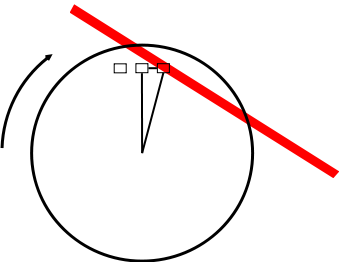
\includegraphics[scale=0.4]{comportamientos/floorSensorsLine.png}
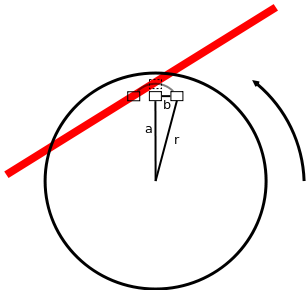
\includegraphics[scale=0.4]{comportamientos/floorSensorsLine1.png}
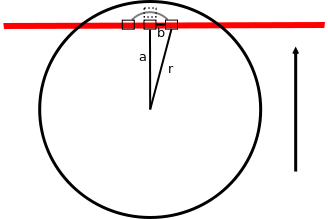
\includegraphics[scale=0.4]{comportamientos/floorSensorsLine2.png}
\caption{Posibles estados iniciales de entrar a la l\'inea}
\label{fig:floorSensorsStates}
\end{center}
\end{figure}


% Explicar el porque del recorrido de la distancia 
% Relacionarlo con la figura fig:floorSensors
Luego del posible giro para lograr que el sensor de piso del medio quede sobre
la l\'inea, se recorre una distancia de $Fsd$, en el caso que el robot no haya
girado anteriormente, o $Fsl$ en el caso que s\'i lo haya hecho. El motivo de
este trayecto es que el centro del robot quede sobre la l\'inea, como muestra
la figura \ref{fig:positioned}. De \'esta forma, s\'olo queda girar nuevamente
hacia el \'angulo que se quiera. Si la l\'inea es la izquierda, entonces el
robot deber\'a girar hasta que su orientaci\'on sea $0$, o $\pi$ en el caso
que la l\'inea sea la derecha.

\begin{figure}[htp]
\begin{center}
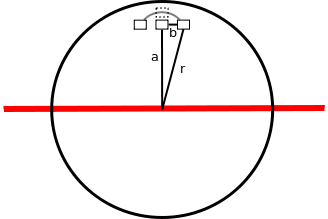
\includegraphics[scale=0.4]{comportamientos/floorSensorsLine3.png}
\caption{Centro del robot sobre la l\'inea y posibles giros}
\label{fig:positioned}
\end{center}
\end{figure}

\paragraph{Seguir l\'inea}
\label{follow_line}
Una vez que el robot est\'a posicionado y con el sensor del medio sobre la
l\'inea, s\'olo basta con seguirla para llegar hacia la zona deseada. \'Este
comportamiento es sencillo de desarrollar.

\subparagraph{Detalle del comportamiento}
Para lograr que el robot siga la l\'inea el objetivo es tratar de mantener
s\'olo el sensor del medio sobre la l\'nea. Entonces, basta con analizar que se
debe hacer en los siguientes casos:
\begin{enumerate}
	\item El sensor de la derecha est\'a sobre la l\'inea
	\item El sensor de la izquierda est\'a sobre la l\'inea
\end{enumerate}
En el primer caso, se debe lograr sacar el sensor de la derecha de la l\'inea,
describiendo un peque\~no arco hacia ese lado. El segundo caso es an\'alogo:
para sacar el sensor de la izquierda de la l\'inea se debe seguir una
trayectoria con un peque\~no \'angulo hacia la izquierda. 

\subparagraph{Implementaci\'on del comportamiento}
El \emph{pseudo-c\'odigo} es simple:
\begin{verbatim}
por cada paso
    veloc_izq = veloc_der = VELOC_SEGUIR_LINEA
    si (esta_en_la_linea(sensor_piso(IZQUIERDA))) entonces
        veloc_izq *= (1 - FACTOR_DE_GIRO)
        veloc_der *= (1 + FACTOR_DE_GIRO)
    fin si
    si (esta_en_la_linea(sensor_piso(DERECHA))) entonces
        veloc_izq *= (1 + FACTOR_DE_GIRO)
        veloc_der *= (1 - FACTOR_DE_GIRO)
    fin si
    poner_velocidades_en_ruedas(veloc_izq,veloc_der)
\end{verbatim}

\subsubsection{Descargar Basura}
\label{unload_garbage}
Una vez que el robot logr\'o llegar a la zona de descarga de basura, debe
descargarla. Para \'esto decidimos ubicar un servo en la parte trasera del
robot, con la misma idea del servo en la parte posterior utilizado para
recolectar.

\paragraph{Detalle del comportamiento}
Para descargar la basura el robot debe posicionarse de forma tal que la
compuerta de descarga quede adyacente a la zona. Dado que para llegar a la
misma el robot sigui\'o la l\'inea, al finalizar va a estar orientado con un
\'angulo en un entorno de $\frac{\pi}{2}$, mirando la zona de descarga. Como el
servo de descarga se encuentra en la parte trasera, deber\'a realizar un giro
para luego poder descargar la basura.
\paragraph{Implementaci\'on del comportamiento}
\begin{verbatim}
    posicionarse()
    levantar(servo_trasero)
    recorrerdistancia(ANCHO_ROBOT)
    cerrar(servo_trasero)
\end{verbatim}

\subsubsection{Ir a base de recarga de bater\'ia}
\label{go_to_recharge}
Ayudados por la elecci\'on que tomamos de poner la zona de descarga de basura
muy cercana a la zona donde se recarga la bater\'ia, decidimos utilizar la
misma estrategia de seguir la l\'inea para llegar hacia la misma.
\\
La diferencia
entre ambos casos es el est\'imulo ante el cual se activan. En el caso de
ir a la zona de descarga, el est\'imulo proviene del sensor del dep\'osito
interno de basura que indica que el mismo est\'a lleno. En el caso de ir
a la base de recarga de bater\'ia, el est\'imulo para la activaci\'on depende
de los valores de dos sensores de bater\'ia que indican bater\'ia baja:
\begin{itemize}
	\item El sensor de la bater\'ia del robot, de donde se alimentan los sensores,
			actuadores y motores.
	\item El sensor de la computadora que corre el controlador.
\end{itemize}

\subsubsection{Cargar Bater\'ia}
\label{recharge_battery}
\paragraph{Detalle del comportamiento}
\paragraph{Implementaci\'on del comportamiento}
\begin{verbatim}
    posicionarse()
    mientras(bateria_no_llena(BATERIA_ROBOT)
            o bateria_no_llena(BATERIA_PC)) hacer

        esperar()
    fin mientras
\end{verbatim}

\begin{comment}

\subsubsection{Recalibrarse}
\label{recalibrate}
\paragraph{Detalle del comportamiento}
\paragraph{Implementaci\'on del comportamiento}

\end{comment}

\subsubsection{Evitar Obst\'aculos}
\label{avoid_obstacles}
\emph{Evitar obst\'aculos} es uno de los comportamientos con mayor jerarqu\'ia
en la arquitectura que elegimos. Su nivel se debe a la importancia que tiene
en un ambiente estructurado pero din\'amico como es el elegido. El objetivo
del robot es facilitar una tarea, sin entorpecer el tr\'ansito de personas.
\\
\paragraph{Detalle del comportamiento}
Para lograr tener conocimiento sobre la proximidad de un obst\'aculo, utilizamos
sensores de proximidad explicados en \ref{sensores de proximidad}.
Dependiendo de la proximidad sensada por un sensor, el robot deber\'a alejarse
de ese lado para evitar un posible choque. La activaci\'on del comportamiento
depender\'a entonces de un valor menor del sensor que haga que la distancia
hacia un obst\'aculo lleve al robot a quedarse estancado o le imposibilite
moverse.
\paragraph{Implementaci\'on del comportamiento}
La implementaci\'on de \'este comportamiento la hicimos utilizando una
red neuronal sin capas ocultas (ver figura \ref{fig:redN}) usando los sensores
de distancia como entradas y las 2 neuronas de salida indicando los valores a
ser seteados a los motores de las ruedas.
\\
Notar que hay conexiones tanto inhibitorias como excitatorias. Como es de
esperarse, ambos sensores traseros (4 y 5) exitan a ambos motores. Distinto es
el caso de los sensores del lado izquierdo (5, 6 y 7) que exitan el motor
ubicado de su lado e inhiben el motor del lado opuesto, de forma tal que el
robot gire para el lado opuesto de la ubicaci\'on de los sensores. La misma
idea se sigue con los sensores (0, 1 y 2) ubicados en el costado derecho del
robot.
\\
Luego de entrenar la red, obtuvimos los siguientes valores para los pesos de la
misma:

\begin{table}[ht]
	\begin{center}
		\begin{tabular}{ | c | c | c | c | c | c | c | c | c | }
			\hline 
			Rueda & $W_0$ & $W_1$ & $W_2$ & $W_3$ &  $W_4$ & $W_5$ & $W_6$ & $W_7$ \\
			\hline\hline
			Izquierda & -0.9 & -0.85 & -0.2 & 0.6 & 0.5 & 0.35 & 0.8 & 0.6 \\
			\hline
			Derecha & 0.9 & 0.85 & 0.2 & 0.6 & 0.5 & -0.35 & -0.8 & -0.6 \\
			\hline
		\end{tabular}
	\end{center}
	\label{pesos_obstaculo} 
	\caption{Asignaci\'on de pesos para evitar obst\'aculos}
\end{table}
Se puede ver que los pesos que influyen en el motor de una rueda influyen
con igual fuerza pero distinto signo en el motor de la rueda contraria.
\\
Este comportamiento, en \emph{pseudo-codigo} puede verse como:
\begin{verbatim}
por cada paso
    veloc_izq = suma(coeficiente(RUEDA_IZQ)(SENSOR_I) * VALOR(SENSOR_I))
    veloc_izq *= FACTOR_DE INCIDENCIA
    veloc_der = suma(coeficiente(RUEDA_DER)(SENSOR_I) * VALOR(SENSOR_I))
    veloc_der *= FACTOR_DE INCIDENCIA
    poner_velocidades_en_ruedas(veloc_izq,veloc_der)
\end{verbatim}

\begin{figure}[htp]
\begin{center}
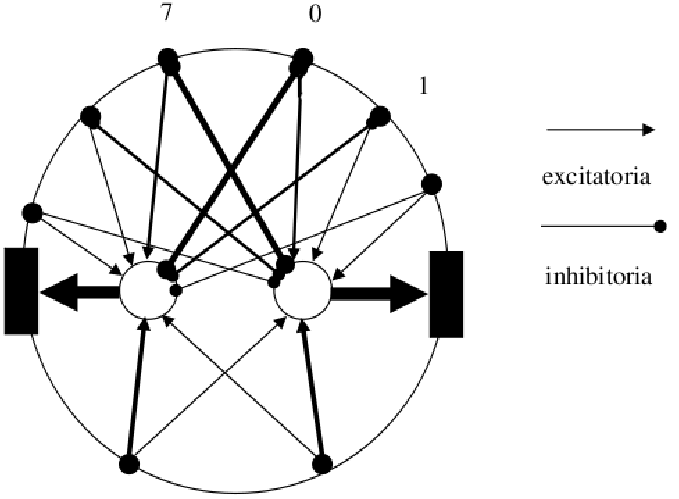
\includegraphics[scale=0.4]{comportamientos/red.png}
\caption{Red neuronal entre los sensores de distancia y los motores}
\label{fig:redN}
\end{center}
\end{figure}

\subsubsection{Salir de situaciones no deseadas}
\label{out_of_unwanted_situations}
\emph{Salir de situaciones no deseadas} surgi\'o como un comportamiento
para ayudar al objetivo de la autonom\'ia del robot. A medida que fuimos
corriendo las simulaciones, observamos que hab\'ia situaciones donde corr\'ia
peligro la autonom\'ia del robot. Un ejemplo de estas situaciones es el caso
donde se ``activan mutuamente'' entre dos comportamientos.
\\
Para ver esto m\'as claramente, supongamos dos comportamientos $A$ y $B$ con
nivel en la jerarqu\'ia $N(A)$ y $N(B)$, siendo $N(A) > N(B)$. Si la respuesta
a un est\'imulo de $A$ lleva a la activaci\'on de $B$ y a la desactivaci\'on de
$A$ y luego la respuesta de $B$ lleva a la activaci\'on de $A$, podr\'ia llegar
a entrarse en un ciclo si es que esta situaci\'on se da por un tiempo
prolongado. El mayor peligro para la autonom\'ia se corre cuando $A$ es el
comportamiento de \emph{evitar obst\'aculos} y $B$ es el comportamiento de
\emph{ir a zona de recarga de bater\'ia} ya que el robot podr\'ia terminar
qued\'andose sin bater\'ia en ese ciclo.
\paragraph{Detalle del comportamiento}
Las situaciones no deseadas se dan la mayor\'ia de los casos cuando un
comportamiento hace girar al robot hacia un lado y el otro comportamiento hacia
el lado contrario, aproximadamente en la misma magnitud. \'Esto quiere decir
que la posici\'on del robot se mantiene alrededor de un punto por un per\'iodo
prolongado de tiempo, por lo que decidimos tomar este hecho como est\'imulo
para la activaci\'on de este comportamiento.
\\
La respuesta del comportamiento es, entonces, girar un \'angulo que cambie la
direcci\'on del robot y adem\'as, que la suma de esa magnitud no sea
peri\'odica.
\'Esta \'ultima condici\'on se pide por el siguiente escenario:
\begin{itemize}
	\item Los comportamientos $A$ y $B$ se ``activan mutuamente'' cuando la
		orientaci\'on del robot es $0$.
	\item Los comportamientos $C$ y $D$ se ``activan mutuamente'' cuando la
		orientaci\'on del robot es $\pi$.
	\item La respuesta de \emph{salir de situaciones no deseadas} es girar un
		\'angulo $\pi$.
\end{itemize}

\paragraph{Implementaci\'on del comportamiento}
\begin{verbatim}
    angulo_actual = obtener_angulo_actual(odometria)
    nuevo_angulo = angulo_actual + ANGULO_A_SUMAR
    girar(nuevo_angulo)
\end{verbatim}



\newpage
\subsection{Odometr\'ia}
\label{odometry}
Para saber donde se encuentra el robot en cierto momento utilizamos \\
odometr\'ia. Esta t\'ecnica se basa en la medici\'on del encoder en cuentas
realizadas por cada motor para obtener el desplazamiento realizado por la
rueda asociada.
\\
A diferencia de los m\'etodos de posicionamiento absoluto, la odometr\'ia
da una estimaci\'on del desplazamiento \emph{local} a la ubicaci\'on anterior
del robot, por lo cual \emph{un error} en una estimaci\'on \emph{se propaga}
hacia las siguientes estimaciones. 
\\
Para calcular la posici\'on $P_n$ en el instante de tiempo n y la orientaci\'on
$O_n$ en base a la posici\'on $P_{n-1}$ en el instante (n-1) y
la correspondiente orientaci\'on $O_{n-1}$, usamos las siguientes f\'ormulas:
\begin{eqnarray}
\label{eqn:left_enc_diff}
d_l = \frac{(e_l(n) - e_l(n-1)) * R_l}{EncRes} \\
\label{eqn:right_enc_diff}
d_r = \frac{(e_r(n) - e_r(n-1)) * R_r}{EncRes} \\
lc = \frac{d_r + d_l}{2} \\
P_n = P_{n-1} + (lc * \cos{O_{n-1}}\textbf{,}lc * \sin{O_{n-1}}) \\
O_n = O_{n-1} + \frac{d_r - d_l}{dbw}
\end{eqnarray}
donde $d_l$ y $d_r$ son las distancias recorridas por las ruedas izquierda y
derecha respectivamente. Ambas son calculadas teniendo en cuenta los valores
anteriores y actuales de los encoders $e_i(n)$, el radio de la rueda $R_i$,
la resoluci\'on del encoder $EncRes$ y es la distancia entre ruedas $dbw$.
\\
Los errores que influyen en el c\'alculo de la odometr\'ia pueden ser de dos
tipos:

\begin{itemize}

\item{Sistem\'aticos:} Son aquellos que pueden ser corregidos o tenidos en
cuenta para disminuir el error.

\item{No sistem\'aticos:} Son aquellos que pueden intentarse corregir pero
\emph{no} eliminar.

\end{itemize}

Decidimos tener en cuenta dos errores sistem\'aticos para disminuir el error
en la odometr\'ia :
\begin{itemize}
\item{Incerteza sobre la distancia entre las ruedas ($dbw$)}
\item{Ruedas con radios diferentes ($R_l$ y $R_r$)}
\end{itemize}
Tuvimos en cuenta estos errores dado que son los que m\'as contribuyen al error
acumulado a lo largo del trayecto del robot.
Para corregir estas fuentes de error, utilizamos el \emph{test del camino
bidireccional describiendo un cuadrado} (UMBmark)
\footnote{http://www-personal.umich.edu/~johannb/Papers/umbmark.pdf}. Dado que
en el momento de realizar el test no ten\'iamos un robot f\'isico, decidimos
realizar el test sobre un e-puck simulado en Webots. As\'i fuimos obteniendo
los valores de correcci\'on para los di\'ametros de las ruedas $c_i$ y la
correci\'on sobre la distancia entre las ruedas $c_{dbw}$ hasta que el error
sistem\'atico m\'aximo dejara de disminuir. En la figura \ref{fig:errsist}
mostramos c\'omo disminuye el error a lo largo de las iteraciones.

\begin{figure}[htp]
\begin{center}
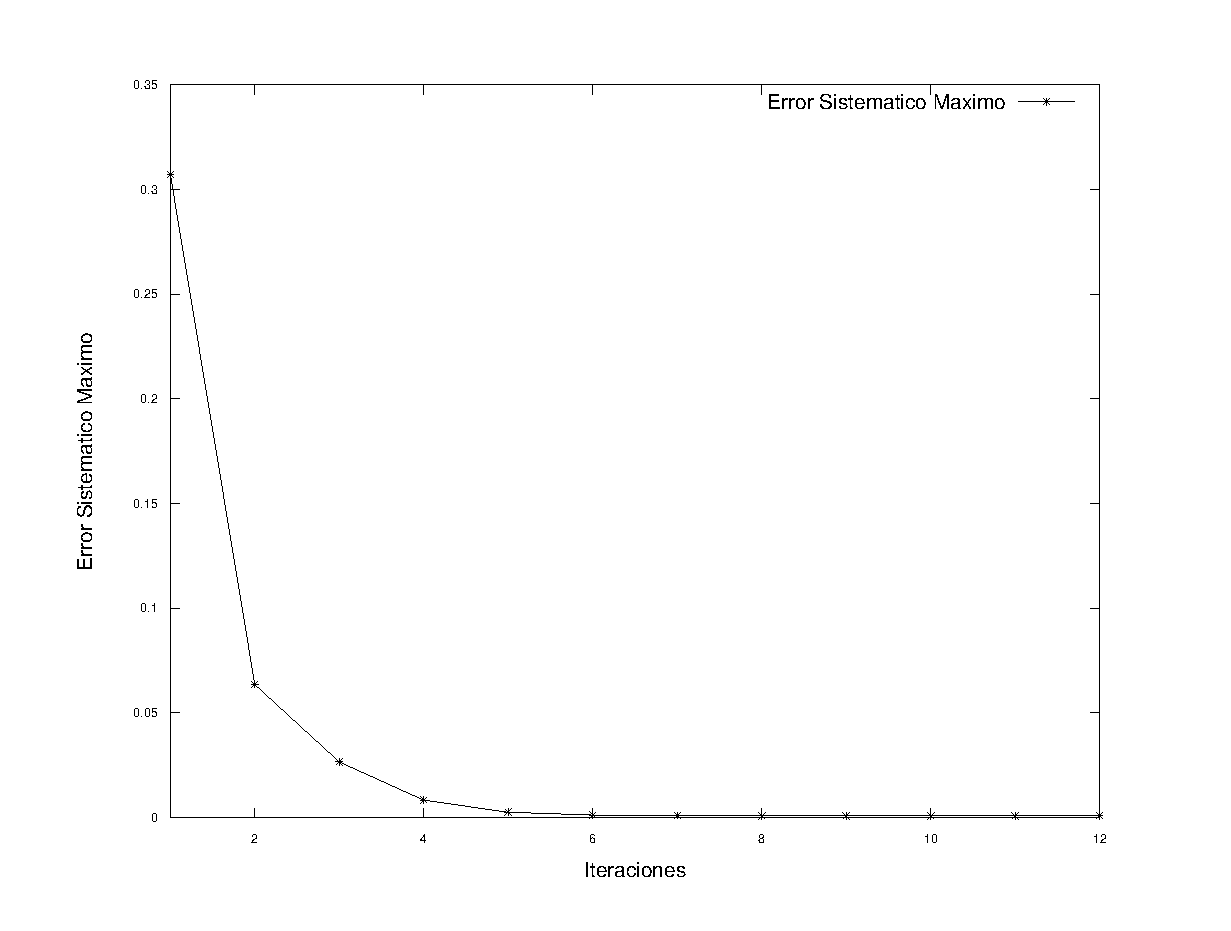
\includegraphics[scale=0.6]{comportamientos/figures/errsist.eps}
%
\includegraphics[scale=0.3]{comportamientos/figures/unk.jpg}
\caption{Error Sistem\'atico M\'aximo a lo largo de las iteraciones}
\label{fig:errsist}
\end{center}
\end{figure}

En la \'ultima iteraci\'on obtuvimos los coeficientes de correcci\'on
$c_l = 0.99998703$, $c_r = 1.00001297$ y $c_{dbw} = 1.092171094$ para ruedas
con radio $R_l = R_r = 0.205$, una distancia entre ruedas de $0.052$ y una
resoluci\'on de encoder $EncRes = 159.23$.

\subsubsection{Problemas con la odometr\'ia}
\label{odometry:problems}
En las simulaciones previas a la presentada en la secci\'on \ref{results}
observamos que el comportamiento emergente del robot no era el esperado.
Viendo m\'as en detalle, el robot tomaba decisiones err\'oneas en los
comportamientos que utilizaban la odometr\'ia. Despu\'es de una extensiva
revisi\'on de c\'odigo, llegamos a la conclusi\'on que el mismo no ten\'ia
problemas.
\\\indent
Fue entonces que decidimos agregar un GPS(con error m\'inimo y que luego
eliminamos) al e-puck en la simulaci\'on con Webots, con el objetivo de
obtener un gr\'afico que indique el error en la odometr\'ia a lo largo de la
simulaci\'on. El resultado esperado era que la odometr\'ia inicie con un error
cercano a 0 y vaya creciendo constantemente a medida que avanzaba la
simulaci\'on. El resultado no fue el esperado pero si iluminativo: el
crecimiento era en partes constante, pero hab\'ia momentos en los cuales
crec\'ia abruptamente.
\\\indent
Decidimos entonces simular nuevamente y ver que comportamiento estaba activo
en dichos momentos. Nos sorprendi\'o ver que en esos momentos el
comportamiento activo era \emph{Evitar obst\'aculos} ya que era uno de los
m\'as simples y de los que m\'as ten\'iamos confianza que no haya un error
de l\'ogica de c\'odigo. Nuevamente revisamos el c\'odigo, sin encontrar
problemas.
\\\indent
\'Esto nos llev\'o a pensar qu\'e relaci\'on hab\'ia entre \emph{Evitar
obst\'aculos} y la odometr\'ia. El comportamiento setea velocidades en las
ruedas y la odometr\'ia utiliza los valores de los encoders de las ruedas.
Revisando las ecuaci\'ones \ref{eqn:left_enc_diff} y \ref{eqn:right_enc_diff}
nos dimos cuenta de lo siguiente: dado que las correcciones $c_l$ y $c_r$
de los radios $R_l$ y $R_r$ de las ruedas minimizan el error pero no lo
eliminan, el error de las ecuaciones aumenta proporcionalmente a la diferencia
entre $e_i(n)$ y $e_i(n-1)$. Y \'esto suced\'ia cuando se activaba el
evitamiento de obst\'aculos ya que daba velocidades a las ruedas de un orden
de magnitud mayor a los que ten\'ian anteriormente.
\\\indent
Finalmente, teniamos que buscar una soluci\'on a \'este problema, ya sabiendo
la verdadera causa del mismo. Pensamos en dos opciones:
\begin{enumerate}
	\item{}Disminuir las velocidades que \emph{Evitar obst\'aculos} asignada
			 a las ruedas, dividi\'endolas por una cte.
	\item{}Hacer que cada vez que se setee una velocidad, se haga un
			c\'alculo con la velocidad seteada anteriormente, de forma tal que
			no haya saltos de \'ordenes de magnitud.
\end{enumerate}
Por el tiempo que dispon\'iamos en ese momento y por simplicidad y r\'apidez
de implementaci\'on, elegimos la primer opci\'on. Cabe aclarar que la segunda
opci\'on es m\'as abarcativa y robusta, ya que sirve para cualquier
comportamiento. Sin embargo, es invasiva en parte ya que puede que el
desarrollador quiera, por alg\'un motivo, que haya ese tipo de variaciones y
no va a poder lograrlo.

\newpage
\subsection{Interfaces con hardware y m\'odulo de reconocimiento de objetos}
\label{interfaces}
Decidimos hacer que el controlador encargado de realizar los comportamientos
sea independiente de la forma con la que se implemente el hardware y el
reconocimiento de los objetos. Para \'esto definimos
interfaces para la comunicaci\'on entre el controlador y el hardware y el
m\'odulo de reconocimiento de objetos de forma tal que los dos \'ultimos puedan
cambiar su implementaci\'on pero brindando siempre la informaci\'on que necesita
el controlador para poder realizar los comportamientos. Esta decisi\'on nos
posibilit\'o realizar un controlador que sea capaz de ser ejecutado tanto en
Webots, donde se hizo el desarrollo, como en la base real del robot. Cabe
aclarar que el traspaso de la simulaci\'on a la realidad no es instant\'anea,
ya que hay que calibrar los dispositivos y realizar nuevamente la odometr\'ia,
entre otras cosas, pero el trabajo demandado es mucho menor ya que una
correcci\'on en la l\'ogica de los comportamientos se puede observar tanto en
un simulador como en la realidad.

\subsubsection{Interfaz con hardware}
La interfaz con el hardware se basa en tener clases encargadas de obtener los
valores de los sensores o del accionar de los actuadores.
\\En la implementaci\'on de la interfaz que corrimos en Webots, hicimos
llamadas al controlador del simulador, que utiliza sensores y actuadores
simulados.
\\En la implementaci\'on que se comunica con el robot f\'isico,
las llamadas las hicimos a un servidor encargado de enviar y recibir paquetes
del protocolo descripto en la secci\'on \ref{h_comm} a trav\'es del puerto
serial.
\\De esta forma es cuesti\'on de decidir que implementaci\'on se usa en base
a si se quiere correr en un simulador como Webots o en el robot f\'isico. Si
quisi\'eramos usar otro simulador u otro tipo de hardware, s\'olo har\'ia falta
que implementemos la interfaz que cumpla con lo establecido e indicarle a la
capa de comportamientos que la utilice para realizar su ejecuci\'on.

\subsubsection{Interfaz con m\'odulo de reconocimiento de objetos usando
Visi\'on}
Como el controlador de comportamientos es \textbf{cliente} del m\'odulo de\\
reconocimiento, necesita conocer en el instante de tiempo $t$, que objetos
est\'an siendo reconocidos. Para esto el m\'odulo debe tener una fuente de
informaci\'on, en nuestro caso, una c\'amara usada para Visi\'on.
\\
Desde el punto de vista anat\'omico, \'esto se puede ver como los ojos
(c\'amara), la parte del cerebro encargada de analizar el est\'imulo recibido
(im\'agenes) por los mismos (m\'odulo de reconocimiento) y la parte del cerebro
encargada de analizar los est\'imulos recibidos y realizar las acciones
(controlador de comportamientos). Si hubi\'esemos usado alg\'un tipo de
conjunto de sensores t\'actiles para reconocer objetos (mano), en vez de
visi\'on, el m\'odulo de reconocimiento de objetos bien podr\'ia analizar la
informaci\'on que ellos proveen e informar al controlador sobre su an\'alisis.
\\
Esta analog\'ia puede llevar a pensar que los sensores de distancia u otros
dispositivos que usamos en este desarrollo bien podr\'ian formar parte de otro
m\'odulo, y no se estar\'ia equivocado. La raz\'on por la cual el m\'odulo de
visi\'on est\'a separado y el resto de los sensores no, es que el procesamiento
de una secuencia de im\'agenes es muy complejo y demandante, tal como detallamos
en la secci\'on \ref{sec:vision}.

\newpage
\subsection{Resultados obtenidos}
\label{results}
En esta secci\'on describimos los par\'ametros que utilizamos en la
simulaci\'on para obtener los resultados sobre los diferentes
comportamientos. Luego presentamos dichos resultados y extraemos
conclusiones sobre los mismos.
\\
A lo largo del proceso de desarrollo fuimos realizando diferentes
simulaciones, de las cuales observamos defectos en las implementaciones de los
comportamientos as\'i como retardos y detalles que pod\'iamos mejorar en
algunos y que fuimos corregiendo. \\
La arena utilizada en dichas simulaciones la mostramos en la figura
\ref{fig:arena_sim}. A lo largo de la misma hay ubicados 15 objetos que simulan
ser basuras, un \'area de recarga de bater\'ia y un \'area de descarga de
basura, marcadas por el cilindro naranja. Los valores de los par\'ametros
que utilizamos  los detallamos en el cuadro \ref{sim_params}. Los \'angulos
los expresamos en radianes y las distancias las expresamos en metros, as\'i
como tambi\'en los radios, correcciones y separaciones. La resoluci\'on de la
c\'amara la expresamos en pixeles, la de la grilla en unidades y los tiempos
est\'an en milisegundos.
\begin{table}[ht]
	\begin{center}
		\begin{tabular}{|c|c|c|c|c|c|c|c|c|}
			\hline
			Par\'ametro & Descripci\'on del par\'ametro & Valor \\
			\hline
			$P_r(0)$ & Posici\'on Inicial del robot & (-0.295,-0.4) \\
			$O_r(0)$ & Orientaci\'on Inicial del robot & 0 \\
			$R_r$ & Radio del robot & 0.026 \\
			$dbw$ & Distancia entre ruedas & 0.052 \\
			$c_{dbw}$ & Correcci\'on de la distancia entre ruedas & 1.09217109 \\
			$R_l$ & Radio de la rueda izquierda & 0.0205 \\
			$R_r$ & Radio de la rueda derecha & 0.0205 \\
			$c_l$ & Correcci\'on del radio de la rueda izquierda & 0.99998702 \\
			$c_r$ & Correcci\'on del radio de la rueda derecha & 1.00001297 \\
			$EncRes$ & Resoluci\'on del encoder & 159.23 \\
			$Cd$ & Distancia de la c\'amara al centro del robot & 0.0355 \\
			$Ch$ \'o $C_h$ & Altura de la c\'amara & 0.038 \\
			$FOV_h$ & Field of view horizontal & 1.1 \\
			$ac$ & \'Angulo de la c\'amara & -0.5 \\
			$C_{rw}$ & Ancho de la im\'agen obtenida de la c\'amara & 640 \\
			$C_{rh}$ & Alto de la im\'agen obtenida de la c\'amara & 480 \\
			$A_w$ & Ancho del arena & 2 \\
			$A_h$ & Alto del arena & 1.2 \\
			$A_{rw}$ & Ancho de la grilla & 100 \\
			$A_{rh}$ & Alto de la grilla & 38 \\
			$Fsd$ & Dist. s.de piso del medio al centro del robot & 0.03 \\
			$Fss$ & Separaci\'on entre sensores de piso & 0.01 \\
			$\delta_f$ & \'Angulo umbral de basura enfocada & 0.1 \\
			$Ts$ & Time Step & 32 \\
			\hline
		\end{tabular}
	\end{center}
	\caption{Par\'ametros utilizados para las simulaciones}
	\label{sim_params}
\end{table}

\begin{figure}[htp]
\begin{center}
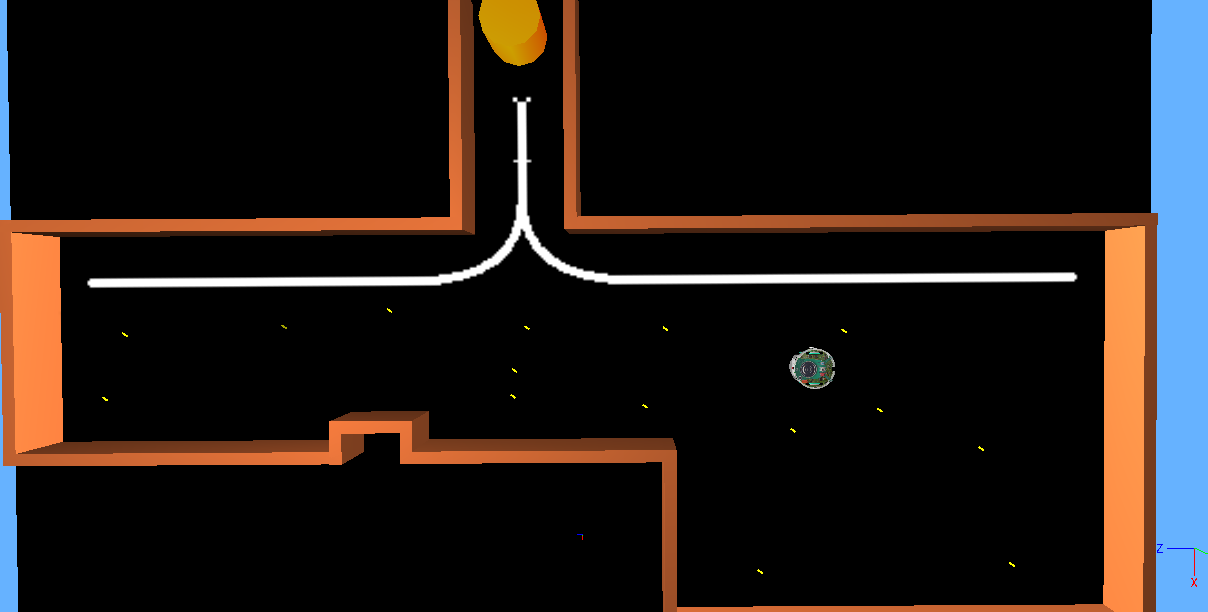
\includegraphics[scale=0.25]{comportamientos/figures/arenaSim.png}
\caption{Arena que utilizamos para las simulaciones}
\label{fig:arena_sim}
\end{center}
\end{figure}

%\subsubsection{Tiempo promedio en recolectar basura}
%Calcular t min, con un escenario donde las basuras las pongo apenas sale de la
%base
%Calcular t max, con un escenario donde las basuras estan lo m\'as lejos de la
%base posible

%\subsubsection{Tiempo promedio de wandering}
%(Tiempo en que est\'a activo el wandering)/(Tiempo total de simulaci\'on)

%\subsubsection{Distribuci\'on de tiempos entre los diferentes comportamientos}
%(tiempo de comportamiento i)/(Tiempo total de simulaci\'on)

%\subsubsection{Relaci\'on (t\_cargando + t\_ir a base) / tiempo total}
%T busqueda basura/ (t a base + tiempo carga bateria + t salir base)

%\subsubsection{Porcentaje de espacio cubierto}

\subsubsection[Distribuci\'on y progreso de comportamientos]{Distribuci\'on de
			tiempos y progreso de comportamientos en la simulaci\'on}
En la figura \ref{fig:behaviourDistribution} mostramos la distribuci\'on
de time steps en la simulaci\'on de cada comportamiento. Podemos ver que
\emph{Recargar bater\'ia} y \emph{Descargar basura} en conjunto est\'an
activos el $54\%$ de la simulaci\'on. Los comportamientos involucrados en la
recolecci\'on de basura (\emph{Enfocar basura}, \emph{Ir a basura} y
\emph{Recolectar basura}) abarcan el $10.5\%$ del tiempo total de
simulaci\'on. El $35.5\%$ restante est\'a repartido en los comportamientos
encargados de una navegaci\'on libre de obst\'aculos y situaciones peligrosas
(\emph{Wandering}, \emph{Evitar obst\'aculos} y \emph{Salir de situaciones no
deseadas}). Todos los comportamientos relacionados con la basura(desde que se
detecta hasta que se descarga) abarcan un $43\%$ del tiempo total de
simulaci\'on. Tambi\'en se puede observar que el comportamiento que mayor
tiempo est\'a activo a lo largo de la simulaci\'on es \emph{Descargar basura}
y el que menor tiempo est\'a activo es \emph{Salir de situaciones no deseadas}.

\begin{figure}[htp]
\begin{center}
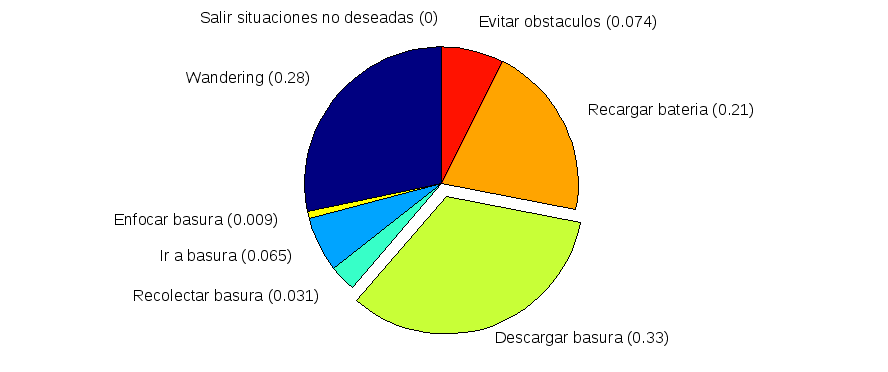
\includegraphics[scale=0.3]{comportamientos/graphics/BehaviourDistributionPieUse.png}
\caption{Distribuci\'on de los tiempos de los comportamientos en la
				simulaci\'on}
\label{fig:behaviourDistribution}
\end{center}
\end{figure}

En la figura \ref{fig:behaviourEvolution} mostramos el progreso a lo largo
de la simulaci\'on de todos los comportamientos. Observamos que en el comienzo
($0 < t < 10000$) \footnote{t es el n\'umero de time step de la simulaci\'on}
la mayor\'ia de los comportamientos est\'a activo aproximadamente la misma
cantidad de time steps, salvando el caso de \emph{Descargar Basura}. En el
per\'iodo ($40000 < t < 50000$), el comportamiento \emph{Wandering} alcanza
a estar activo la misma cantidad de steps que \emph{Ir a basura}. Podemos
ver tambi\'en que la forma en que evolucionan \emph{Enfocar basura},
\emph{Ir a basura} y \emph{Recolectar basura} a lo largo de la simulaci\'on
es muy similar, salvando la cantidad de steps que est\'an activos. La
evoluci\'on de \emph{Recargar bater\'ia} es peri\'odica: inicia con
una meseta de time steps en los cuales no est\'a activo y luego tiene
una pendiente pronunciada. Diferente es el progreso de \emph{Evitamiento
de obst\'aculos} ya que sus mesetas son las menos prolongadas y sus
pendientes son poco abruptas.

\begin{figure}[htp]
\begin{center}
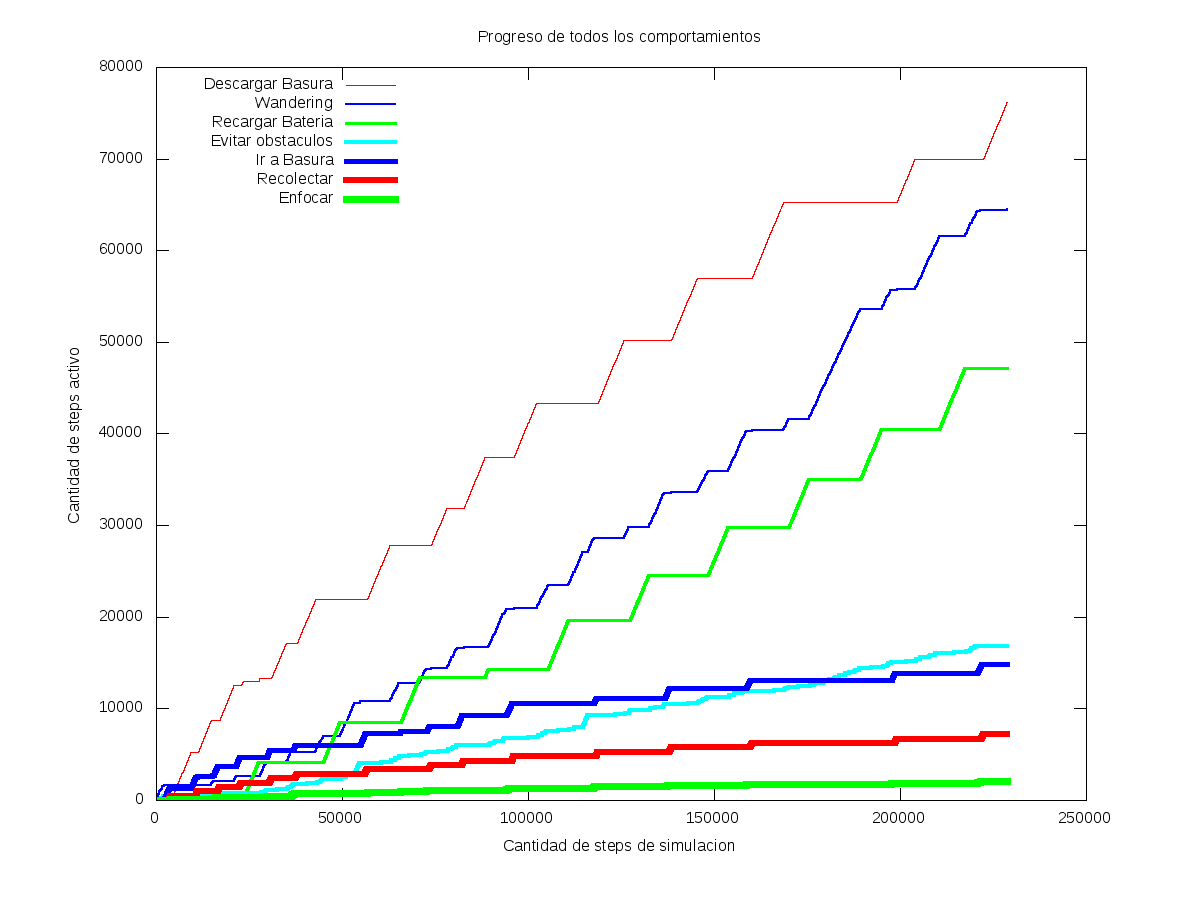
\includegraphics[scale=0.25]{comportamientos/graphics/AllUse.png}
\caption{Evoluci\'on de los comportamientos a lo largo de la simulaci\'on}
\label{fig:behaviourEvolution}
\end{center}
\end{figure}

En la figura \ref{fig:collectEvolution} mostramos m\'as en detalle el
comportamiento vital para nuestro proyecto, \emph{Recolectar basura}. Podemos
ver que en el per\'iodo ($0<t<50000$) acumula aproximadamente la misma
cantidad de steps hechos que en el per\'iodo ($50000<t<150000$). El progreso
describe mesetas cuyas duraciones se van prolongando a medida que se avanza la
simulaci\'on y las pendientes tienen aproximadamente la misma magnitud a lo
largo de la misma.

\begin{figure}[htp]
\begin{center}
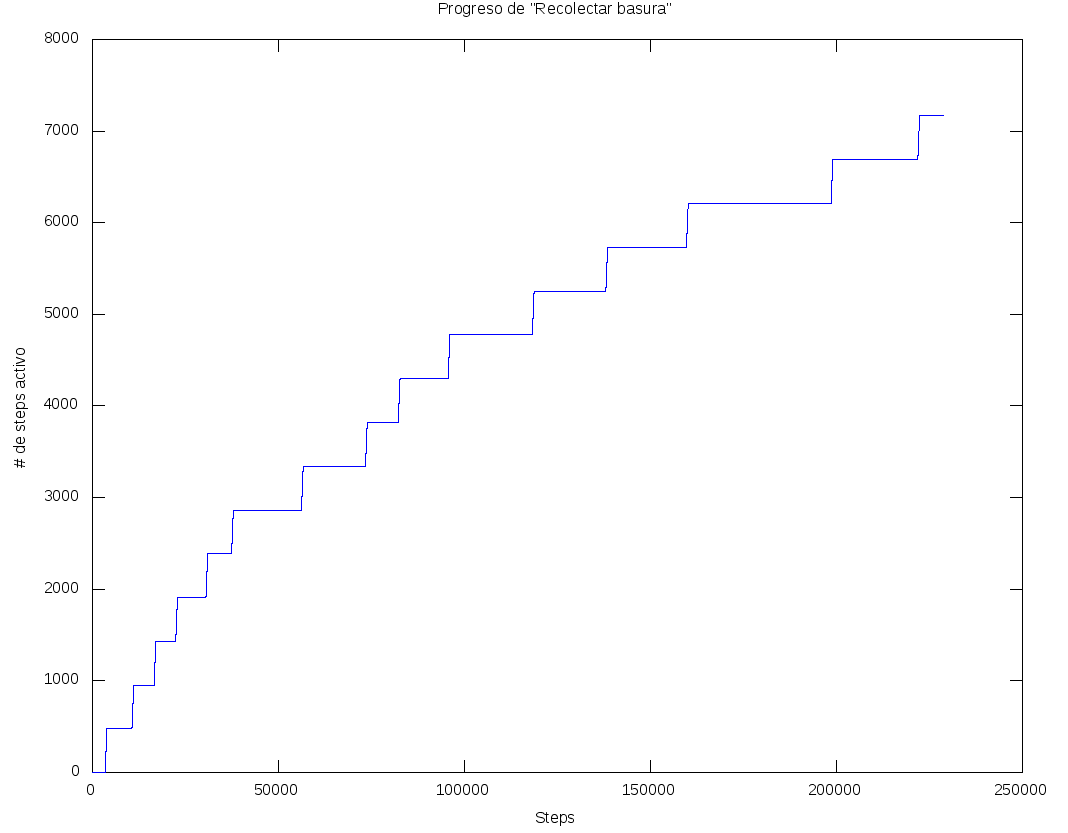
\includegraphics[scale=0.25]{comportamientos/graphics/CollectUse.png}
\caption{Progreso del comportamiento \emph{Recolectar Basura}}
\label{fig:collectEvolution}
\end{center}
\end{figure}

Para que pudieramos ver m\'as en detalle lo que sucedi\'o con los
comportamientos, obtuvimos la cantidad de veces que cada uno se
activ\'o (Ver cuadro \ref{behaviours_stats}). En el mismo observamos
que el comportamiento que m\'as veces se activ\'o fue \emph{Evitar
obst\'aculos}, seguido por \emph{Enfocar basura} y \emph{Wandering}.
En un orden de magnitud menor est\'an \emph{Ir a descargar basura} e
\emph{Ir a recargar bater\'ia}. Finalmente, \emph{Recolectar basura}
se activ\'o 15 veces y \emph{Salir de situaciones indeseadas} nunca.

\begin{table}[htp]
	\begin{center}
		\begin{tabular}{|c|c|c|}
			\hline
			Comportamiento & \# total de steps activo
							& \# veces que se activ\'o \\
			\hline
			Wandering & 64476 & 1330 \\
			Enfocar basura & 2057 & 1384 \\
			Ir a basura & 14832 & 1218 \\
			Recolectar basura & 7166 & 15 \\
			Ir a descargar basura & 76160 & 321 \\
			Ir a recargar bater\'ia & 47188 & 265 \\
			Evitar obst\'aculos & 16843 & 1507 \\
			Salir situaciones indeseadas & 0 & 0 \\
			\hline
		\end{tabular}
	\end{center}
	\caption{Resultados sobre steps en los cuales los comportamientos est\'an
					activos}
	\label{behaviours_stats}
\end{table}

\subsubsection[Tiempos en $caa$ y $cai$ de comportamientos]{Tiempos en que
			los comportamientos est\'an continuamente activos e inactivos}
En los cuadros \ref{behaviours_stats_active} y \ref{behaviours_stats_inactive} mostramos
c\'alculos sobre los steps que cada comportamiento estuvo $caa$
\footnote{caa: continuamente activo. Por continuamente activo se entiende que
estuvo activo en el time step $t-1$ y en el $t$} y $cai$ \footnote{cai: 
continuamente inactivo. Por continuamente inactivo se entiende que no estuvo
activo en el timestep $t-1$ ni en el $t$}, respectivamente.
\\\indent
Podemos ver que \emph{Recolectar basura} es en promedio el mayor en ambos
cuadros y que tiene el menor desv\'io est\'andar en $caa$. \emph{Wandering} es
en promedio el que menor tiempo est\'a $cai$, con el segundo menor desv\'io.
Sucede lo mismo con \emph{Evitar obst\'aculos}, segundo en promedio en estar
$cai$ y con el menor desv\'io. Ambos, adem\'as, tienen los m\'inimos m\'aximos
en estar $cai$, con una diferencia de un orden de magnitud con respecto al
resto de los comportamientos. \emph{Ir a descargar basura} e \emph{Ir a
recargar bater\'ia} son de los que mayor promedio y desv\'io tienen tanto en
estar $caa$ como en estar $cai$. Los comportamientos de \emph{Enfocar basura}
y \emph{Ir a basura} tienen un promedio y desv\'io est\'andar de los m\'as
bajos en estar $caa$.

\begin{table}[htp]
	\begin{center}
		\begin{tabular}{|c|c|c|c|}
			\hline
			Comportamiento & Promedio & Desv\'io Est\'andard & \# m\'aximo \\
			\hline
			Wandering & 48.44 & 225.07 & 2212 \\
			Enfocar basura & 1.48 & 3.27 & 67 \\
			Ir a basura & 12.17 & 58.44 & 1222 \\
			Recolectar basura & 477.73 & 0.70 & 478 \\
			Ir a descargar basura & 237.25 & 840.49 & 6012 \\
			Ir a recargar bater\'ia & 178.06 & 647.39 & 3950 \\
			Evitar obst\'aculos & 11.17 & 54.72 & 1386 \\
			Salir situaciones indeseadas & - & - & - \\
			\hline
		\end{tabular}
	\end{center}
	\caption{Resultados sobre steps que los comportamientos est\'an continuamente
					activos}
	\label{behaviours_stats_active}
\end{table}

\begin{table}[htp]
	\begin{center}
		\begin{tabular}{|c|c|c|c|}
			\hline
			Comportamiento & Promedio & Desv\'io Est\'andard & \# m\'aximo \\
			\hline
			Wandering & 123.4 & 754.4 & 8351 \\
			Enfocar basura & 163.7 & 1766 & 38000 \\
			Ir a basura & 175.5 & 1811 & 38040 \\
			Recolectar basura & 13850 & 9479 & 38400 \\
			Ir a descargar basura & 473.8 & 2689 & 30520 \\
			Ir a recargar bater\'ia & 682.5 & 3322 & 23270 \\
			Evitar obst\'aculos & 140.5 & 724.3 & 9485 \\
			Salir situaciones indeseadas & - & - & - \\
			\hline
		\end{tabular}
	\end{center}
	\caption{Resultados sobre steps que los comportamientos est\'an continuamente
					inactivos}
	\label{behaviours_stats_inactive}
\end{table}

\subsubsection[Transiciones entre comportamientos]{Transiciones hacia y desde
			un comportamiento a otro}
En el cuadro \ref{transitions} mostramos las transiciones entre los
comportamientos. \'Estos est\'an abreviados y presentados en el mismo
orden que en la secci\'on \ref{comportamientos}. El valor en la posici\'on
$(i$,$j) = t_{ij}$, siendo $i$ y $j$ el n\'umero de fila y columna
respectivamente, se lee como: ``desde el comportamiento $i$ se pas\'o
$t_{ij}$ veces al comportamiento $j$''. Tambi\'en se puede leer como:
``el comportamiento $j$ se activ\'o $t_{ij}$ veces siendo el
comportamiento $i$ el que anteriormente estaba activo''. Consideramos
que hay una transici\'on cuando $i \neq j$, por lo que $t_{ii} = 0$. Una
transici\'on de $i$ a $j$ con $i > j$ puede ser porque el est\'imulo necesario
para la activaci\'on del comportamiento $i$ ya no est\'a presente. Una
transici\'on de $i$ a $j$ con $i < j$ puede ser porque el est\'imulo necesario
para la activaci\'on del comportamiento $j$ pas\'o a ser sensado.
\\\indent
El comportamiento que m\'as veces ``activ\'o'' a otro comportamiento es
\emph{Enfocar basura}, activando a \emph{Ir a basura}. Observamos tambi\'en
que el caso contrario es la 2da transici\'on m\'as hecha y ambos valores
est\'an relativamente cercanos. El caso que los valores de $t_{ij}$ y $t_{ji}$
est\'en cercanos tambi\'en sucede con \emph{Evitar}\\
\emph{obst\'aculos} y el resto
de los comportamientos, aunque en estos casos la diferencia es mucho menor.
\\\indent
Podemos ver que hay transiciones que s\'olo se dan 1 sola vez. \'Estas son:
\begin{itemize}
	\item{}\emph{Wandering} a \emph{Recolectar basura},
	\item{}\emph{Enfocar basura} a \emph{Descargar basura} e
	\item{}\emph{Ir a basura} a \emph{Recargar bater\'ia}
\end{itemize}

\begin{table}[htp]
	\begin{center}
		\begin{tabular}{|c||c|c|c|c|c|c|c|}
		\hline
    	 & W & EB & IAB & RB & DB & R & EO \\
		\hline
		\hline
			W & $0$ & $303$ & $176$ & $1$ & $12$ & $5$ & $833$ \\
		\hline
			EB & $238$ & $0$ & $1036$ & $2$ & $1$ & $0$ & $107$ \\
		\hline
			IAB & $229$ & $967$ & $0$ & $12$ & $2$ & $1$ & $7$ \\
		\hline
			RB & $12$ & $3$ & $0$ & $0$ & $0$ & $0$ & $0$ \\
		\hline
			DB & $14$ & $0$ & $0$ & $0$ & $0$ & $2$ & $305$ \\
		\hline
			R & $9$ & $0$ & $0$ & $0$ & $1$ & $0$ & $255$ \\
		\hline
			EO & $828$ & $111$ & $6$ & $0$ & $305$ & $257$ & $0$ \\
		\hline
		\end{tabular}
	\end{center}
	\caption{Transiciones entre comportamientos}
	\label{transitions}
\end{table}

Mostramos tambi\'en las transiciones en forma de porcentajes en los cuadros
\ref{transitions_percentages} y \ref{transitions_percentages_ret}. En el
primero detallamos las transiciones desde $i$ hacia $j$ y en el segundo,
transiciones de $j$ hacia $i$. Se puede ver que las transiciones que m\'as
sucedieron fueron desde \emph{Descargar basura} y \emph{Recargar bater\'ia}
hacia \emph{Evitar obst\'aculos}, con un porcentaje mayor al $95\%$, y que
el segundo tambi\'en es la causa principal de la activaci\'on de los primeros,
con porcentajes de $95\%$ y $97\%$ respectivamente.
\\\indent
En segundo lugar se ubican las transiciones desde \emph{Enfocar basura} hacia
\emph{Ir a basura} y el rec\'iproco, con valores cercanos al $75\%$. Algo
parecido sucede en el segundo cuadro.
\\\indent
El $80\%$ de las veces que estuvo activo \emph{Recolectar basura} luego se
activ\'o \emph{Wandering} y el $80\%$ de las veces que se activ\'o el primero
fue por parte de \emph{Ir a basura}.

\begin{table}[htp]
	\begin{center}
		\begin{tabular}{|c||c|c|c|c|c|c|c|}
		\hline
    	 & W & EB & IAB & RB & DB & R & EO \\
		\hline
		\hline
			W & $0\%$ & $0.227\%$ & $0.132\%$ & $0.001\%$ & $0.009\%$ & $0.003\%$ & $0.626\%$ \\
		\hline
			EB & $0.172\%$ & $0\%$ & $0.748\%$ & $0.002\%$ & $0.001\%$ & $0\%$ & $0.077\%$ \\
		\hline
			IAB & $0.188\%$ & $0.794\%$ & $0\%$ & $0.01\%$ & $0.002\%$ & $0.001\%$ & $0.006\%$ \\
		\hline
			RB & $0.8\%$ & $0.2\%$ & $0\%$ & $0\%$ & $0\%$ & $0\%$ & $0\%$ \\
		\hline
			DB & $0.043\%$ & $0\%$ & $0\%$ & $0\%$ & $0\%$ & $0.006\%$ & $0.951\%$ \\
		\hline
			R & $0.034\%$ & $0\%$ & $0\%$ & $0\%$ & $0.004\%$ & $0\%$ & $0.962\%$ \\
		\hline
			EO & $0.55\%$ & $0.074\%$ & $0.004\%$ & $0\%$ & $0.202\%$ & $0.170\%$ & $0\%$ \\
		\hline
		\end{tabular}
	\end{center}
	\caption{Transiciones desde $i$ hacia $j$ en porcentajes}
	\label{transitions_percentages}
\end{table}

\begin{table}[htp]
	\begin{center}
		\begin{tabular}{|c||c|c|c|c|c|c|c|}
		\hline
    	 & W & EB & IAB & RB & DB & R & EO \\
		\hline
		\hline
			W & $0\%$ & $0.179\%$ & $0.172\%$ & $0.009\%$ & $0.011\%$ & $0.007\%$ & $0.623\%$ \\
		\hline
			EB & $0.219\%$ & $0\%$ & $0.699\%$ & $0.002\%$ & $0\%$ & $0\%$ & $0.08\%$ \\
		\hline
			IAB & $0.145\%$ & $0.851\%$ & $0\%$ & $0\%$ & $0\%$ & $0\%$ & $0.004\%$ \\
		\hline
			RB & $0.066\%$ & $0.134\%$ & $0.8\%$ & $0\%$ & $0\%$ & $0\%$ & $0\%$ \\
		\hline
			DB & $0.037\%$ & $0.003\%$ & $0.006\%$ & $0\%$ & $0\%$ & $0.003\%$ & $0.95\%$ \\
		\hline
			R & $0.019\%$ & $0\%$ & $0.003\%$ & $0\%$ & $0.008\%$ & $0\%$ & $0.97\%$ \\
		\hline
			EO & $0.553\%$ & $0.071\%$ & $0.004\%$ & $0\%$ & $0.202\%$ & $0.170\%$ & $0\%$ \\
		\hline
		\end{tabular}
	\end{center}
	\caption{Transiciones desde $j$ hacia $i$ en porcentajes}
	\label{transitions_percentages_ret}
\end{table}

\subsubsection[Arena recorrida]{Progreso de recorrido de la arena a lo largo de
			la simulaci\'on}

En la figura \ref{fig:seenArea} mostramos el progreso del \'area recorrida por
el robot a lo largo de la simulaci\'on. El arena estaba dividida en
$A_{rw}$.$A_{rh} = 3800$ slots. Como es de esperarse, la suma de cantidad de
slots vistos y slots restantes en un instante de tiempo $t$ es $cte=3800$. El
tiempo en que se lleg\'o a recorrer todo el arena fue $t_{fv} = 95241$. Dado
que la duraci\'on de la simulaci\'on fue de $t_{fs} = 228721$, el arena se
recorri\'o en el $0.42\%$ del tiempo total de simulaci\'on.
\\\indent
Se puede ver que al principio de la simulaci\'on ($0<t<17000$) hay pendientes
abruptas, con mesetas de pocos steps. Luego las pendientes tienen menor valor
y las mesetas son m\'as prolongadas, salvando el caso del intervalo
($35000<t<40000$).

\begin{figure}[htp]
\begin{center}
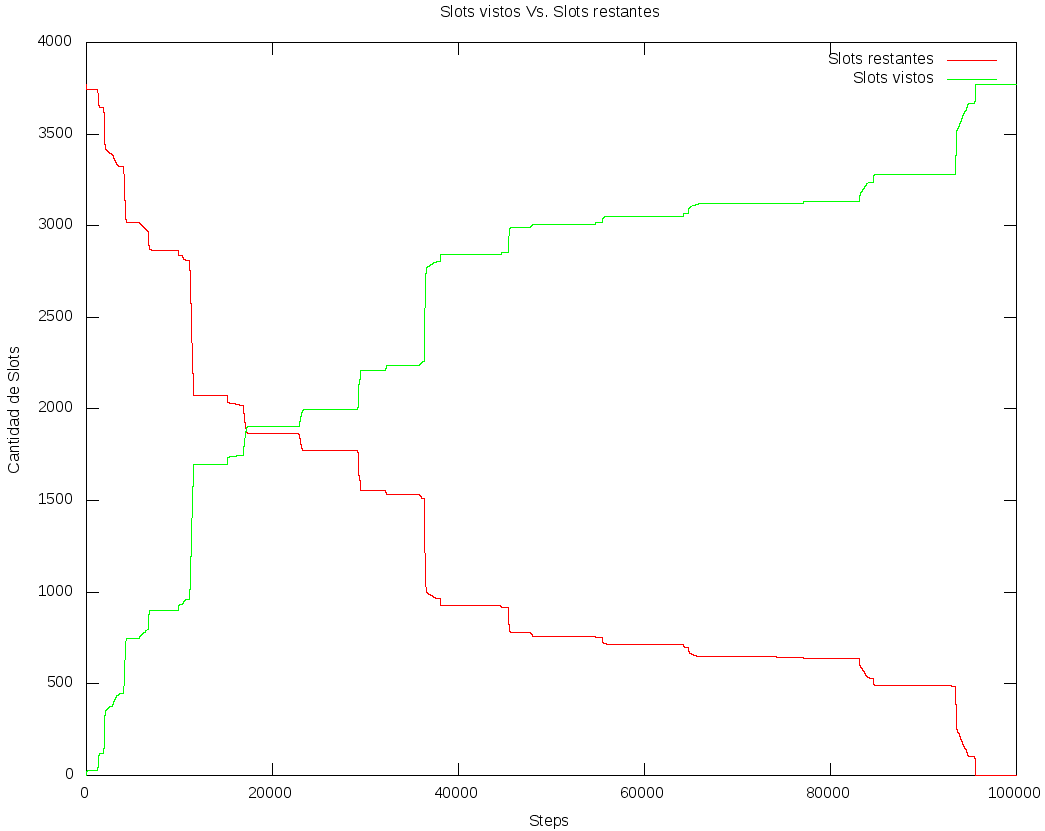
\includegraphics[scale=0.25]{comportamientos/graphics/areaCoveredVsTimeUse.png}
\caption{\'Area visualizada y \'area no visualizada a lo largo de la
				simulaci\'on}
\label{fig:seenArea}
\end{center}
\end{figure}

En el cuadro \ref{arena:covered} vemos m\'as en detalle el progreso del
porcentaje de arena cubierto. Tomamos 10 muestras uniformes en el per\'iodo
($0<t<t_{fv}$) y obtuvimos el porcentaje cubierto en esa muestra, as\'i
como tambi\'en el acumulado la misma. Podemos ver que ya en la 2da muestra,
$0<t<0.042 t_{fs}$, se alcanza a recorrer el $50\%$ del total del arena.
Despu\'es los incrementos son m\'as peque\~nos en comparaci\'on a los primeros,
salvando el caso de la cuarta y \'ultima muestra. En la primer muestra el
robot recorri\'o aproximadamente el $25\%$ de la arena, en la segunda el $50\%$
y en la cuarta el $75\%$.

%esp_cub / (e\sp_cub + esp_nocub)
\begin{table}[htp]
	\begin{center}
		\begin{tabular}{|c||c|c|}
		\hline
			$N^\circ$ muestra & (\%) & (\%) Acumulado \\
		\hline
			1 & 0.246 & 0.246 \\
		\hline
			2 & 0.258 & 0.505 \\
		\hline
			3 & 0.081 & 0.586 \\
		\hline
			4 & 0.167 & 0.754 \\
		\hline
			5 & 0.044 & 0.798 \\
		\hline
			6 & 0.011 & 0.809 \\
		\hline
			7 & 0.017 & 0.827 \\
		\hline
			8 & 0.003 & 0.830 \\
		\hline
			9 & 0.038 & 0.869 \\
		\hline
			10 & 0.130 & 1 \\
		\hline
		\end{tabular}
	\end{center}
	\caption{Porcentaje de arena cubierta}
	\label{arena:covered}
\end{table}

\newpage
\subsection{Conclusi\'on}
\label{comp_conclusion}
En \'esta secci\'on sacamos conclusiones sobre los resultados obtenidos en la
secci\'on \ref{results}, as\'i como dar posibles explicaciones a los mismos.
\\\indent
Dado que en la simulaci\'on hab\'ia 15 basuras, era esperado que
\emph{Recolectar basura} se activase la misma cantidad de veces. En promedio,
el robot recolect\'o
\begin{equation*}
	\frac{t_{fs}}{15 basuras} = \frac{1.52x10^5 Ts}{basura}
\end{equation*}
es decir, 1 basura cada 8 minutos. El mayor tiempo que pas\'o entre
entre una recolecci\'on y otra fue de $38400 Ts = 20 m 28 s$.
\\\indent
Los comportamientos \'intimamente relacionados, \emph{Enfocar basura} e
\emph{Ir a basura} se activaron m\'as de 15 veces. Ambos comportamientos
tuvieron un nivel de activac\'ion parecido a la cantidad de steps que
estuvieron activos, provocando un bajo promedio de steps $caa$. \'Esto pudo
haber sido causado debido al umbral $\delta_f$ en el cual se decide si una
basura est\'a enfocada o no(ver figura \ref{fig:focusAngles}). Un valor muy
grande del mismo, figura (a), cubre m\'as porcentaje de la im\'agen, por lo que
va a llevar a indicar que la basura se enfoca m\'as r\'apido, disminuyendo el
tiempo en que el comportamiento est\'a activo. Un valor chico (figura (b)),
har\'a que la mayor cantidad de veces que se detecte una basura, la misma
no est\'e enfocada y al cubrir menos porci\'on de la im\'agen, aumentar\'a
el promedio de time steps en los cuales tiene que enfocar. \'Este caso
es m\'as sensible a la situaci\'on en la que la basura se mueve, ya que
va a ocasionar que se tenga que enfocar nuevamente. El primer caso es
menos sensible al movimiento de la basura, pero tiene el siguiente defecto:
cuando la basura se sensa como enfocada, la misma \emph{NO} est\'a frente
al robot, y el comportamiento de \emph{Ir a basura} s\'olo va hacia adelante,
suponiendo que la basura se encuentra frente al robot, ocasionando que la
basura pase a no estar enfocada y una nueva activaci\'on de \emph{Enfocar
basura}. En los cuadros de transiciones \ref{transitions_percentages} y
\ref{transitions_percentages_ret} podemos ver que ambos comportamientos
son los mayores proveedores de transiciones de dichos estados al otro.
\\\indent
Como ya mencionamos, \emph{Ir a descargar basura} e \emph{Ir a recargar
bater\'ia} en conjunto abarcan el $54\%$ del tiempo total de simulaci\'on.
Adem\'as son de los que mayor promedio est\'an $caa$, lo que nos
lleva a pensar que una activaci\'on incorrecta de los mismos es indeseable,
ya que son de los que m\'as jerarqu\'ia tienen y por lo tanto inhibir\'ian
innecesariamente y por un tiempo relativamente prolongado a otros. Una
activaci\'on incorrecta puede estar dada por:
\begin{itemize}
	\item{} Mal funcionamiento de los sensores
	\item{} Haber juntado un objeto que no era basura
	\item{} Una falla en la l\'ogica de activaci\'on de comportamientos
\end{itemize}
El gran desv\'io est\'andar de ambos en $caa$ se debe a que su acci\'on es
llevar al robot hacia las l\'ineas, y la distancia y el recorrido por las
mismas var\'ia seg\'un la posici\'on del robot cuando se hizo presente el
est\'imulo correspondiente.
\\\indent
El promedio en estar $cai$ de \emph{Ir a descargar basura} depende
directamente de la cantidad de basuras que haya en la arena y la efectividad
del m\'odulo de reconocimiento. En el caso que no haya basuras en la arena,
lo ideal es que el comportamiento nunca se active, aunque \'esto depende de
las posibles activaciones incorrectas. El gran desvi\'o est\'andar en estar
$cai$ se debe a que al principio de la simulaci\'on hab\'ia m\'as basuras
para recolectar, disminuyendo el tiempo entre activaci\'ones, y llegando al
final de la simulaci\'on hab\'ia menos basuras, disminuyendo la probabilidad
que el robot las encuentre y aumentando el tiempo entre activaciones.
%Aca puedo hablar del cai de ir a recargar basura tambien
\\\indent
Los valores de \emph{Wandering} dependen totalmente de las activaciones de los
otros comportamientos, ya que est\'a activo si y s\'olo si ning\'un otro
est\'a activo. En un arena con 15 basuras, estuvo activo un $28\%$ del tiempo
de simulaci\'on. Teniendo en cuenta que los comportamientos relacionados con
las basuras abarcaron un $43\%$ de $t_{fs}$, es de esperarse que en una
simulaci\'on sin basuras el protagonismo de \emph{Wandering} sea el mayor
de todos superando el $70\%$. Su bajo promedio y desv\'io est\'andar en estar
$cai$ puede estar dado por situaciones en que est\'a activo, un comportamiento
pasa a estar activo por un per\'iodo corto de tiempo(por ejemplo, \emph{Evitar
obst\'aculos}, que causa el $62\%$ de activaciones) hasta que desaparece el
est\'imulo que lo activ\'o y el robot vuelve a hacer \emph{Wandering}. En la
mayor parte de los casos entre una activaci\'on y otra de \emph{Wandering} no
hay muchos comportamientos que se activan.
%Se podria hacer un cuadro con la cantidad de comportamientos que se activan
%entre una activacion y otra de un comportamiento
\\\indent
\emph{Evitar obst\'aculos} es un comportamiento que tiene ciertas cualidades.
Una de ellas se puede ver en los cuadros de transiciones. Las transiciones
hacia \'el y desde \'el se dan en proporciones muy parecidas, esto quiere decir
que $t^1_{7j} \approx t^2_{7j}$, siendo $t^1$ y $t^2$ transiciones de los
cuadros \ref{transitions_percentages} y \ref{transitions_percentages_ret}
respectivamente.
\\\indent
\'Esto da la siguiente idea: hay un comportamiento activo $A$ y sus respuestas
est\'an llevando al robot a una posible colisi\'on. En ese momento se activa
\emph{Evitar obst\'aculos}, detiene $A$, saca al robot de la posible colisi\'on
y vuelve a activar a $A$. Cabe aclarar que en realidad no lo activa a $A$, sino
que desaparece el est\'imulo de \emph{Evitar obst\'aculos} y $A$ toma el
control nuevamente. Su promedio y desv\'io estandar de $caa$ son bajos y se ven
reflejados en la figura \ref{fig:behaviourEvolution}. En la misma figura se
puede observar el efecto de tener un promedio y desv\'io estandar bajos,
reflejados en la duraci\'on muy corta de las mesetas. El poder de detener a
otros comportamientos est\'a dado por su nivel en la arquitectura. Es
importante resaltar que este beneficio viene solo por el hecho de usar
\emph{Subsumption}, y en el caso de haber utilizado otra arquitectura, nos
hubiese demandado trabajo.
\\\indent
El comportamiento de \emph{Salir de situaciones no deseadas} no se activ\'o
nunca. \'Este hecho es muy importante: indica que el resto de los
comportamientos nunca se ``activaron mutuamente'' y por lo tanto no hubo
situaciones que puedan llevar al robot a quedarse sin carga en la bater\'ia,
arriesgando su autonom\'ia. El hecho que no se active nunca el comportamiento
puede llevar a pensar que no es necesario tenerlo. \'Este pensamiento es
totalmente err\'oneo ya que uno de nuestros objetivos era que la autonom\'ia
del robot no corra riesgo bajo ning\'un concepto. Cabe aclarar que hay
situaciones que escapan al alcance de este proyecto, por ejemplo, que se
rompa una rueda.
\\\indent
El funcionamiento de \emph{Salir de situaciones no deseadas} lo probamos
en diferentes simulaciones anteriores a la que presentamos y el resultado
fue el esperado.
\\\indent
%Hablar de los odd cases
En la secci\'on \ref{results} vimos que algunas transiciones suced\'ian s\'olo
una vez. A continuaci\'on detallamos posibles causas de las mismas:
\begin{enumerate}
	\item{}\emph{Wandering} a \emph{Recolectar basura},
	\item{}\emph{Enfocar basura} a \emph{Descargar basura} e
	\item{}\emph{Ir a basura} a \emph{Recargar bater\'ia}
\end{enumerate}
El primer caso puede estar dado por el siguiente escenario:
\begin{itemize}
	\item{} El robot esquiv\'o un obst\'aculo.
	\item{} En el time step que desapareci\'o ese est\'imulo, hab\'ia una
		basura en la imagen detectada por la c\'amara.
	\item{} En dicho time step, el sistema de reconocimiento no la detect\'o,
		activando \emph{Wandering}.
	\item{} En el siguiente time step, el sistema de reconocimiento detecta la
		basura, y adem\'as se encuentra enfocada y a una distancia en la cual
		puede activarse el comportamiento de \emph{Recolectar basura}.
\end{itemize}
El segundo caso puede estar dado por el siguiente escenario:
\begin{itemize}
	\item{} El robot recolect\'o una basura.
	\item{} En el time step que se desactiv\'o la recolecci\'on, hab\'ia otra
		basura en la imagen detectada por la c\'amara y por el sistema de
		reconocimiento que era necesario enfocar para que sea recolectada,
		pero la basura recolectada no hab\'ia llegado a activar el sensor del
		dep\'osito de basura. Est\'o llev\'o a la activaci\'on de
		\emph{Enfocar basura}.
	\item{} En el siguiente time step, la basura recolectada activa el sensor
		del dep\'osito y por ende, activa el comportamiento \emph{Descargar
		basura}.
\end{itemize}
El tercer caso es m\'as sencillo de explicar:
\begin{itemize}
	\item{} En el time step $t$ el robot se dirig\'ia hacia una basura.
	\item{} En el time step $t+1$, el valor de la bater\'ia hizo que se active
		el comportamiento de \emph{Recargar bater\'ia}. \'Esto es posible
		debido a que el \'ultimo tiene mayor nivel en la arquitectura que el
		primero.
\end{itemize}
Otro dato curioso es que el $80\%$ de las veces que estuvo activo
\emph{Recolectar basura} luego se activ\'o \emph{Wandering} y
el restante a \emph{Enfocar basura}. Teniendo un almacenamiento m\'aximo de
1 basura, es de esperarse que luego de recolectar, se active \emph{Descargar
basura}. \'Esto no sucede ya que, como explicamos en el escenario del segundo
caso, hay un per\'iodo de time steps en los cuales la basura recolectada
est\'a yendo hacia el sensor del dep\'osito, permitiendo la activaci\'on
de otros comportamientos.
\\\indent
Finalmente, el robot recorri\'o toda la arena en el $42\%$ del tiempo total
de simulaci\'on. \'Este porcentaje disminuye o aumenta dependiendo de si
aumenta el tiempo de simulaci\'on o disminuye. Es decir, lo importante no
es el porcentaje del tiempo total, sino el tiempo en que recorri\'o el \'area
en su totalidad. Dicho tiempo fue de $95241Ts = 50m47s$. Durante \'este tiempo
el robot no s\'olo recorri\'o un poco menos de $200m^2$ (la escala es 10:1),
sino que recolect\'o 9 basuras de las 15 que hab\'ia en la arena y fue a
descargarlas(uno de los comportamientos que m\'as tiempo lleva). Adem\'as,
se recarg\'o 3 veces en ese per\'iodo, como dijimos anteriormente, es otro
de los comportamientos que m\'as tiempo demanda. Otro factor importante para
destacar es que el $75\%$ del \'area se recorri\'o en un cuarto del tiempo
en cuesti\'on, es decir, en aproximadamente $13mins$. Por todo \'esto,
concluimos que el recorrido de la arena es muy eficiente.

\subsubsection{Posibles extensiones}
Una de las posibles extensiones del trabajo puede ser minimizar el tiempo
consumido por los comportamientos de \emph{Ir a zona de descarga de basura}
y \emph{Ir a zona de recarga de bater\'ia}. Dado que ambos van hacia la l\'inea,
podemos pensar en algunas formas para minimizar este tiempo. Entre las mismas
est\'an: cambiar las ubicaciones de las l\'ineas, agregar m\'as l\'ineas o
cambiar las formas de las mismas. Otra alternativa podr\'ia ser utilizar otro
mecanismo para ir hacia dichas zonas que no use el seguimiento de l\'inea, o
lo use en menor tiempo. Cabe aclarar que no es el seguimiento de la l\'inea
lo que m\'as tiempo demora sino ir hacia la misma.
\\\indent
En cuanto a los comportamientos que posee el robot podemos pensar en agregar
algunos para ampliar las prestaciones que puede brindar el robot. Entre ellos
se encuentran:
\begin{itemize}
	\item{} Seguir la pared, con un objetivo a pensar.
	\item{} Interactuar con las personas, mediante sonidos o reconociemiento
			visual.
	\item{} Agregar un mecanismo que le permita recolectar basuras que est\'an
			pegadas o en lugares no alcanzables por el robot por la presencia
			de obst\'aculos.
	\item{} Mover una basura hacia un \'area, en caso que no pueda recolectarla.
	\item{} Notificar a una central sobre sucesos inesperados o dif\'iciles
			de que sucedan.
	\item{} Proveer una interfaz web que permita ver el estado de los sensores
			y actuadores del robot en forma on-line, as\'i como tambi\'en
			gr\'aficos mostrando los \'ultimos comportamientos activos. Adem\'as
			podr\'ia ver el estado actual del sistema de predicci\'on y la
			imagen vista por la c\'amara.
	\item{} Subir estad\'isticas a un servidor central de forma tal que se
			pueda analizar qu\'e cambios se podr\'ian hacer en el controlador
			para mejorar la efectividad y eficiencia de la recolecci\'on o
			de otros comportamientos.
\end{itemize}





